% Options for packages loaded elsewhere
\PassOptionsToPackage{unicode}{hyperref}
\PassOptionsToPackage{hyphens}{url}
\PassOptionsToPackage{dvipsnames,svgnames,x11names}{xcolor}
%
\documentclass[
  12pt]{article}

\usepackage{booktabs}
\usepackage{xr-hyper}
\usepackage{graphicx}
\usepackage{amsmath,amssymb,amsthm}
\usepackage{iftex}
\usepackage{placeins}
\ifPDFTeX
  \usepackage[T1]{fontenc}
  \usepackage[utf8]{inputenc}
  \usepackage{textcomp} % provide euro and other symbols
\else % if luatex or xetex
  \usepackage{unicode-math}
  \defaultfontfeatures{Scale=MatchLowercase}
  \defaultfontfeatures[\rmfamily]{Ligatures=TeX,Scale=1}
\fi
\usepackage{lmodern}
\ifPDFTeX\else  
    % xetex/luatex font selection
\fi
% Use upquote if available, for straight quotes in verbatim environments
\IfFileExists{upquote.sty}{\usepackage{upquote}}{}
\IfFileExists{microtype.sty}{% use microtype if available
  \usepackage[]{microtype}
  \UseMicrotypeSet[protrusion]{basicmath} % disable protrusion for tt fonts
}{}
\makeatletter
\@ifundefined{KOMAClassName}{% if non-KOMA class
  \IfFileExists{parskip.sty}{%
    \usepackage{parskip}
  }{% else
    \setlength{\parindent}{0pt}
    \setlength{\parskip}{6pt plus 2pt minus 1pt}}
}{% if KOMA class
  \KOMAoptions{parskip=half}}
\makeatother
\usepackage{xcolor}
\setlength{\emergencystretch}{3em} % prevent overfull lines
\setcounter{secnumdepth}{5}
% Make \paragraph and \subparagraph free-standing
\makeatletter
\ifx\paragraph\undefined\else
  \let\oldparagraph\paragraph
  \renewcommand{\paragraph}{
    \@ifstar
      \xxxParagraphStar
      \xxxParagraphNoStar
  }
  \newcommand{\xxxParagraphStar}[1]{\oldparagraph*{#1}\mbox{}}
  \newcommand{\xxxParagraphNoStar}[1]{\oldparagraph{#1}\mbox{}}
\fi
\ifx\subparagraph\undefined\else
  \let\oldsubparagraph\subparagraph
  \renewcommand{\subparagraph}{
    \@ifstar
      \xxxSubParagraphStar
      \xxxSubParagraphNoStar
  }
  \newcommand{\xxxSubParagraphStar}[1]{\oldsubparagraph*{#1}\mbox{}}
  \newcommand{\xxxSubParagraphNoStar}[1]{\oldsubparagraph{#1}\mbox{}}
\fi
\makeatother


\providecommand{\tightlist}{%
  \setlength{\itemsep}{0pt}\setlength{\parskip}{0pt}}\usepackage{longtable,booktabs,array}
\usepackage{calc} % for calculating minipage widths
% Correct order of tables after \paragraph or \subparagraph
\usepackage{etoolbox}
\makeatletter
\patchcmd\longtable{\par}{\if@noskipsec\mbox{}\fi\par}{}{}
\makeatother
% Allow footnotes in longtable head/foot
\IfFileExists{footnotehyper.sty}{\usepackage{footnotehyper}}{\usepackage{footnote}}
\makesavenoteenv{longtable}
\usepackage{graphicx}
\makeatletter
\def\maxwidth{\ifdim\Gin@nat@width>\linewidth\linewidth\else\Gin@nat@width\fi}
\def\maxheight{\ifdim\Gin@nat@height>\textheight\textheight\else\Gin@nat@height\fi}
\makeatother
% Scale images if necessary, so that they will not overflow the page
% margins by default, and it is still possible to overwrite the defaults
% using explicit options in \includegraphics[width, height, ...]{}
\setkeys{Gin}{width=\maxwidth,height=\maxheight,keepaspectratio}
% Set default figure placement to htbp
\makeatletter
\def\fps@figure{htbp}
\makeatother

\addtolength{\oddsidemargin}{-.5in}%
\addtolength{\evensidemargin}{-.1in}%
\addtolength{\textwidth}{1in}%
\addtolength{\textheight}{1.7in}%
\addtolength{\topmargin}{-1in}
\makeatletter
\@ifpackageloaded{caption}{}{\usepackage{caption}}
\AtBeginDocument{%
\ifdefined\contentsname
  \renewcommand*\contentsname{Table of contents}
\else
  \newcommand\contentsname{Table of contents}
\fi
\ifdefined\listfigurename
  \renewcommand*\listfigurename{List of Figures}
\else
  \newcommand\listfigurename{List of Figures}
\fi
\ifdefined\listtablename
  \renewcommand*\listtablename{List of Tables}
\else
  \newcommand\listtablename{List of Tables}
\fi
\ifdefined\figurename
  \renewcommand*\figurename{Figure}
\else
  \newcommand\figurename{Figure}
\fi
\ifdefined\tablename
  \renewcommand*\tablename{Table}
\else
  \newcommand\tablename{Table}
\fi
}
\@ifpackageloaded{float}{}{\usepackage{float}}
\floatstyle{ruled}
\@ifundefined{c@chapter}{\newfloat{codelisting}{h}{lop}}{\newfloat{codelisting}{h}{lop}[chapter]}
\floatname{codelisting}{Listing}
\newcommand*\listoflistings{\listof{codelisting}{List of Listings}}
\makeatother
\makeatletter
\makeatother
\makeatletter
\@ifpackageloaded{caption}{}{\usepackage{caption}}
\@ifpackageloaded{subcaption}{}{\usepackage{subcaption}}
\makeatother


\ifLuaTeX
  \usepackage{selnolig}  % disable illegal ligatures
\fi
\usepackage[]{natbib}

\usepackage{bookmark}

\IfFileExists{xurl.sty}{\usepackage{xurl}}{} % add URL line breaks if available
\urlstyle{same} % disable monospaced font for URLs
\hypersetup{
  pdftitle={Title},
  pdfauthor={Author 1; Author 2},
  pdfkeywords={3 to 6 keywords, that do not appear in the title},
  colorlinks=true,
  linkcolor={blue},
  filecolor={Maroon},
  citecolor={Blue},
  urlcolor={Blue},
  pdfcreator={LaTeX via pandoc}}

\providecommand{\anon}{0} % default off
\ifnum\anon=1
  % blinded stuff
\else
  % unblinded stuff
\fi


\renewcommand{\thetable}{S\arabic{table}}
\renewcommand{\thefigure}{S\arabic{figure}}
\renewcommand{\theequation}{S\arabic{equation}}
\renewcommand{\thesection}{S\arabic{section}}

%\newtheorem{theorem}{Theorem}



%\title{Supplementary Material for: Z-residuals for Diagnosing Bayesian Models}
%\author{Tingxuan Wu, Effie Gao, Cindy Feng and Longhai Li}




\let\OLDmaketitle\maketitle
\renewcommand{\maketitle}{\begingroup\setstretch{1}\OLDmaketitle\endgroup}

\setlength{\leftmargini}{2.5em}   % level 1
\setlength{\leftmarginii}{1em}% level 2
\setlength{\labelsep}{0.5em}


% 1. Make the "Proof" label bold
\renewcommand{\proofname}{\textbf{Proof:}}

% 2. Create a new counter for steps inside a proof
\newcounter{proofpart}

% 3. Automatically reset the step counter at the start of each proof
\AtBeginEnvironment{proof}{\setcounter{proofpart}{0}}

% 4. Define the custom 'proofpart' environment
\newenvironment{proofpart}[1][]{%
    % This code runs at \begin{proofpart}
    \refstepcounter{proofpart}% Increment the counter
    \par\smallskip\noindent% Start a new paragraph with a small space
    \ifblank{#1}{%
        % If no title is given, just print "Step X."
        \textbf{Step \theproofpart. }\ignorespaces%
    }{%
        % If a title is given, print "Step X (Title)."
        \textbf{Step \theproofpart}~(\textit{#1})\textbf{. }\ignorespaces%
    }%
}{%
    % This code runs at \end{proofpart}
    % The previous \par\medskip was causing the error. Leaving this empty is correct.
}

%%%%%%%%%%%%%%%%%%%%
\usepackage{amsthm}
\theoremstyle{plain}
\newtheorem{theorem}{Theorem}[section]
\newtheorem{lemma}[theorem]{Lemma}
\newtheorem{proposition}[theorem]{Proposition}
\theoremstyle{definition}
\newtheorem{definition}[theorem]{Definition}
\theoremstyle{remark}
\newtheorem{remark}[theorem]{Remark}
\newtheorem{example}[theorem]{Example}


\usepackage{xr-hyper}

\makeatletter
\providecommand{\myexternaldocument}[2][]{%
  \externaldocument[#1]{#2}%
  \IfFileExists{#2.aux}{}{%
    \typeout{No file #2.aux.}%
  }%
}
\makeatother

\IfFileExists{newcommands.tex}{% --- LaTeX Packages ---
% --- LaTeX Packages ---
\usepackage{amsmath}
\usepackage{amsthm}
\usepackage{bm}            % For bold math symbols
\usepackage{graphicx}      % For including images
\usepackage{xcolor}        % Required for \highlight
\usepackage{xspace}        % Required for commands like \nref
\usepackage{tikz}
%\usetikzlibrary{arrows.meta}
%\usepackage{mathtools}
%\usepackage{filecontents}
\usepackage{booktabs}
%\usepackage{placeins}
\usepackage{hyperref}
        \hypersetup{
          colorlinks=true,
          linkcolor=blue,
          urlcolor=blue,
          citecolor=blue
        }
\usepackage{etoolbox}

\setlength{\bibsep}{5pt plus 5pt} % space BETWEEN items
% For tighter lines WITHIN each item:
\usepackage{setspace}
\AtBeginEnvironment{thebibliography}{\setstretch{1.05}}

% --- Custom Commands ---

% Acronyms and Custom Text
\newcommand{\CVIC}{\text{CVIC}}
\newcommand{\deviance}{\text{dev}}
\newcommand{\dpois}{\text{dpois}}
\newcommand{\ic}{\text{ic}}
\newcommand{\nmsp}{\text{\scriptsize NMSP}}
\newcommand{\nrsp}{\text{\scriptsize NRSP}}
\newcommand{\pmin}{p_{\text{\scriptsize min}}}
\newcommand{\pp}{\text{pp}}
\newcommand{\nref}{[\textbf{references}]}
\newcommand{\SP}{survival probability\xspace}
\newcommand{\SPs}{survival probabilities\xspace}
\newcommand{\svf}{S_{i}(\cdot)}
\newcommand{\unif}[0]{\text{Unif}}
\newcommand{\rsp}[0]{\text{RSP}}
\newcommand{\msp}[0]{\text{MSP}}
\newcommand{\PPP}[0]{\text{PPP}}
\newcommand{\PPPs}[0]{\text{PPPs}}
\newcommand{\PPC}[0]{\text{PPC}}
\newcommand{\bU}[0]{\bm{U}}
\newcommand{\pv}[0]{\mathcal{P}}

% Math Symbols (Bold)
\newcommand{\btheta}[0]{\bm{\theta}}
\newcommand{\bTheta}[0]{\bm{\Theta}}
\newcommand{\bx}[0]{\bm{x}}
\newcommand{\by}[0]{\bm{y}}
\newcommand{\bY}[0]{\bm{Y}}
\newcommand{\bbeta}{\bm{\beta}}
\newcommand{\bBeta}{\bm{\Beta}}
\newcommand{\blambda}{\bm{\lambda}}
\newcommand{\bmu}{\bm{\mu}}
\newcommand{\bphi}{\bm{\phi}}
\newcommand{\bp}{\bm{p}}
\newcommand{\bsgm}{\bm{\sigma}}
\newcommand{\hu}[0]{\pi^o_{i}}
\newcommand{\mhu}[0]{\pi^o}
% General Superscripts and Subscripts
\newcommand{\obs}[0]{^{\text{obs}}}
\newcommand{\sobs}[0]{^{\text{obs}}}
\newcommand{\post}[0]{^{\text{Post}}}
\newcommand{\cv}[0]{^{\text{CV}}}
\newcommand{\iscv}[0]{^{\text{ISCV}}}
\newcommand{\supt}[0]{^{(t)}}
\newcommand{\mci}{^{(t)}}        % Kept as it has a different name from \supt
\newcommand{\mcs}{^{(s)}}
\newcommand{\rep}{^{\text{rep}}}
\newcommand{\ppc}{_{\text{ppc}}}
\newcommand{\noi}{_{-i}}
\newcommand{\wi}{_{1:n}}
\newcommand{\IS}{^{\text{\scriptsize IS}}}

% Compound Superscripts for Z-residuals
\newcommand{\rspp}[0]{^{\text{Post-RSP}}}
\newcommand{\mspp}[0]{^{\text{Post-MSP}}}
\newcommand{\rspis}[0]{^{\text{ISCV-RSP}}}
\newcommand{\mspis}[0]{^{\text{ISCV-MSP}}}
\newcommand{\rsppost}{^{\text{Post-RSP }}}  % From first block
\newcommand{\rspiscv}{^{\text{ISCV-RSP}}}    % From first block
\newcommand{\E}{\mathbb{E}}
\newcommand{\Epost}{\mathbb{E}_{\btheta\,|\,\by}}
\newcommand{\Ecv}{\mathbb{E}_{\btheta\,|\,\by_{-i}}}
\newcommand{\highlight}[1]{\textcolor{blue}{#1}}
\newcommand{\pvalue}[0]{$p$-value\xspace}
\newcommand{\pvalues}[0]{$p$-values\xspace}
\newcommand{\norm}[1]{\left\lVert#1\right\rVert}

\newcommand{\textred}[1]{\textcolor{orange}{#1}}


% ===================================================================
%                 THEOREM AND PROOF DEFINITIONS
% ===================================================================



%old theorem style for ba

% % --- 1. Define Custom Theorem Styles ---
% % A style for theorems where the optional note is bold
% \newtheoremstyle{boldnote}
%   {}		    % Space above
%   {}		    % Space below
%   {\itshape}	% Body font
%   {}		    % Indent amount
%   {\bfseries}	% Theorem head font
%   {.}		    % Punctuation after head
%   {.5em}	    % Space after head
%   {\thmname{#1}\thmnumber{ #2}\thmnote{ [\textbf{#3}]}}


% % --- 2. Define Theorem-Like Environments ---
% % Set the default style for all environments defined from this point
% \theoremstyle{plain}

% % The main theorem environment, numbered per section. All others will follow its counter.
% \newtheorem{theorem}{Theorem}[section] 

% % Environments that share the theorem counter
% \newtheorem{lemma}[theorem]{Lemma}
% \newtheorem{corollary}[theorem]{Corollary}

% % Switch to the custom style for any environments you want to use it
% % \theoremstyle{boldnote}
% % \newtheorem{specialtheorem}[theorem]{Special Theorem} % Example


% % --- 3. Define Proof and Step Environments ---
% % For custom "Step" counter within proofs
% \newtheorem{proofpart}{Step}

% % Change the name "Proof" to "Proof" (bold)
% \renewcommand{\proofname}{\textbf{Proof}}

% % Automatically reset the 'Step' counter at the beginning of every proof
% \AtBeginEnvironment{proof}{\setcounter{proofpart}{0}}
% % ===================================================================
}{}

\myexternaldocument[M-]{JASA-template}

%%%%%%%%%%%%%%%%%%%%
%set the key \texttt{anon} to ``0'' to hide the authors and acknowledgements,
%  producing the required anonymized version. 
%Set the key \texttt{anon} to ``1'' to produce the manuscript with author details and
% acknowledgments. 

\begin{document}


\def\spacingset#1{\renewcommand{\baselinestretch}%
{#1}\small\normalsize} \spacingset{1}


%%%%%%%%%%%%%%%%%%%%%%%%%%%%%%%%%%%%%%%%%%%%%%%%%%%%%%%%%%%%%%%%%%%%%%%%%%%%%%
\if1\anon
{
  \title{\bf 
  Supplementary Material for \\ ``Z-residuals for Diagnosing Bayesian Models''
  }
  
\author{%
  Tingxuan Wu\textsuperscript{1},
  Effie Gao\textsuperscript{1},
  Cindy Feng\textsuperscript{2},
  and Longhai Li\textsuperscript{1}\thanks{Corresponding author: \texttt{longhai.li@usask.ca}}\\[1em]
  \textsuperscript{1}Department of Mathematics and Statistics, University of Saskatchewan\\
  \textsuperscript{2}Department of Community Health and Epidemiology, Dalhousie University
}
  \maketitle
} \fi

\if0\anon
{
  \bigskip
  \bigskip
  \bigskip
  \begin{center}
    {\LARGE\bf 

      Supplementary Material for \\ ``Z-residuals for Diagnosing Bayesian Models''

    }
    \today
\end{center}
  \medskip
} \fi

\bigskip

\begin{abstract}
This document contains supplementary simulations, extended applied analyses, and mathematical proofs detailing the theoretical properties of Z-residuals. The material is organized as follows:

\begin{itemize}
    \item \textbf{Section S1 (Additional Simulation Studies):} Presents simulation studies evaluating wrong families (comparing HNB versus NB models) and mixed misspecifications in both families and covariate functional forms. It also provides the full tabular rejection rates for the main-text simulations.
    
    \item \textbf{Section S2 (Additional Results of the Analysis of the Dolphin-Sighting Data):} Details further applied analyses, including posterior summaries for the selected nonlinear HNB model, robustness checks via prior and binning sensitivity analyses, and a numerical illustration of replicated $p$-values.
    
    \item \textbf{Section S3 (Asymptotic Properties of Z-residuals):} Provides the formal theoretical framework, including illustrations and rigorous proofs for the uniformity of Randomised Survival Probabilities (RSPs) under the true model, the asymptotic independence and uniformity of cross-validated and posterior RSPs, the asymptotic uniformity of tests based on Z-residuals, and distribution-free upper bounds for the order statistics of replicated $p$-values.
\end{itemize}
\end{abstract}

               
\spacingset{1.2} % DON'T change the spacing!


\clearpage

\section{\textred{Additional Simulation Studies}}

\subsection{Simulation Studies with Wrong Families: HNB versus NB}\label{simulation_wrong_family}


To assess the capability of the proposed Z-residuals in identifying misspecified distributional families, we conducted a simulation study involving the generation of data from a HNB model, followed by fitting both the true HNB model and a misspecified NB. Each synthetic dataset was constructed by first sampling a covariate $X_i \sim N(0,1)$ and five independent noise covariates $Z_{i,j} \sim N(0,1)$ for $j=1, \dots, 5$. The zero-component probability, $\hu$, was then determined by $\text{logit}(\hu) = \beta_0 + \beta_1 X_i$, and the mean of the count component, $\mu_i$, by $\log(\mu_i) = \alpha_0 + \alpha_1 X_i$, with true regression coefficients set as $\alpha_0 = 2$, $\alpha_1 = 8$, $\beta_0 = -1$, and $\beta_1 = -1$, which were used to generate the final response $y_i \sim \text{HNB}(\mu_i, \hu, \gamma=4)$. We generated 500 datasets for each sample size $n\in\{50,100,200\}$, with an the overall zero proportions $\pi^0 \approx 30\%$. For each simulated dataset, two Bayesian models were fitted using the \texttt{brms} R package: \textbf{the true HNB model}, specified as $y_i \sim \text{HNB}(\mu_i, \hu, \gamma)$ with $\log(\mu_i) = \alpha_0 + \alpha_1 X_i + \sum_{j=1}^5 a_j Z_{i,j}$ and $\text{logit}(\hu) = \beta_0 + \beta_1 X_i + \sum_{j=1}^5 b_j Z_{i,j}$; and \textbf{a misspecified NB model}, formulated as $y_i \sim \text{NB}(\mu_i, \gamma)$ with $\log(\mu_i) = \alpha_0 + \alpha_1 X_i + \sum_{j=1}^5 a_j Z_{i,j}$. The inclusion of noise variables in the linear predictors ensures the models' complexity and a more realistic testing environment for the diagnostic tools.


To demonstrate the performance of Z-residuals as a graphical diagnostic tool, we present scatterplots, QQ and marginal distribution plots in Figure~\ref{fig_scatter_qq_sim1} for a representative dataset with a sample size of $n=100$ and an overall zero proportion of $\mhu\approx 30\%$. 
The three rows provide complementary graphical summaries: the residual-versus-index plots display observation-level residual patterns, the QQ plots assess agreement with the standard normal reference distribution, and the marginal distribution plots show histograms of the Z-residuals with the empirical kernel density and the \(N(0,1)\) reference density overlaid. For the two-part HNB model, the index plots also distinguish zero observations from positive count observations.
When the true HNB model is fitted, the posterior RSP Z-residuals are randomly scattered without any discernible pattern (Figure~\ref{fig_scatter_qq_sim1}(a)). Their corresponding QQ plot aligns well with the diagonal line (Figure~\ref{fig_scatter_qq_sim1}(e)), and their marginal distribution is close to the standard normal reference density (Figure~\ref{fig_scatter_qq_sim1}(i)). The SW test also yields a $p$-value greater than 0.05. This behavior is consistent with the theoretical expectation of a random sample from a standard normal distribution for a correctly specified model. In contrast, the QQ plot for the MSP Z-residuals (Figure~\ref{fig_scatter_qq_sim1}(f)) and its marginal distribution plot (Figure~\ref{fig_scatter_qq_sim1}(j)) deviate visibly from the standard normal reference, resulting in an SW $p$-value of 0.01 that would incorrectly reject the true model. For the misspecified NB model, the QQ plots and marginal distribution plots for the RSP and MSP Z-residuals (Figures~\ref{fig_scatter_qq_sim1}(g), \ref{fig_scatter_qq_sim1}(h), \ref{fig_scatter_qq_sim1}(k), and \ref{fig_scatter_qq_sim1}(l)) exhibit substantial departures from the standard normal reference distribution, with SW $p$-values less than 0.05, clearly indicating poor model fit. These graphical diagnostics show that RSP Z-residuals can distinguish the correctly specified HNB model from the misspecified NB model. Notably, the MSP-based Z-residuals fail to approximate a normal distribution when the data are fitted with the true HNB model.
\begin{figure}[htp]
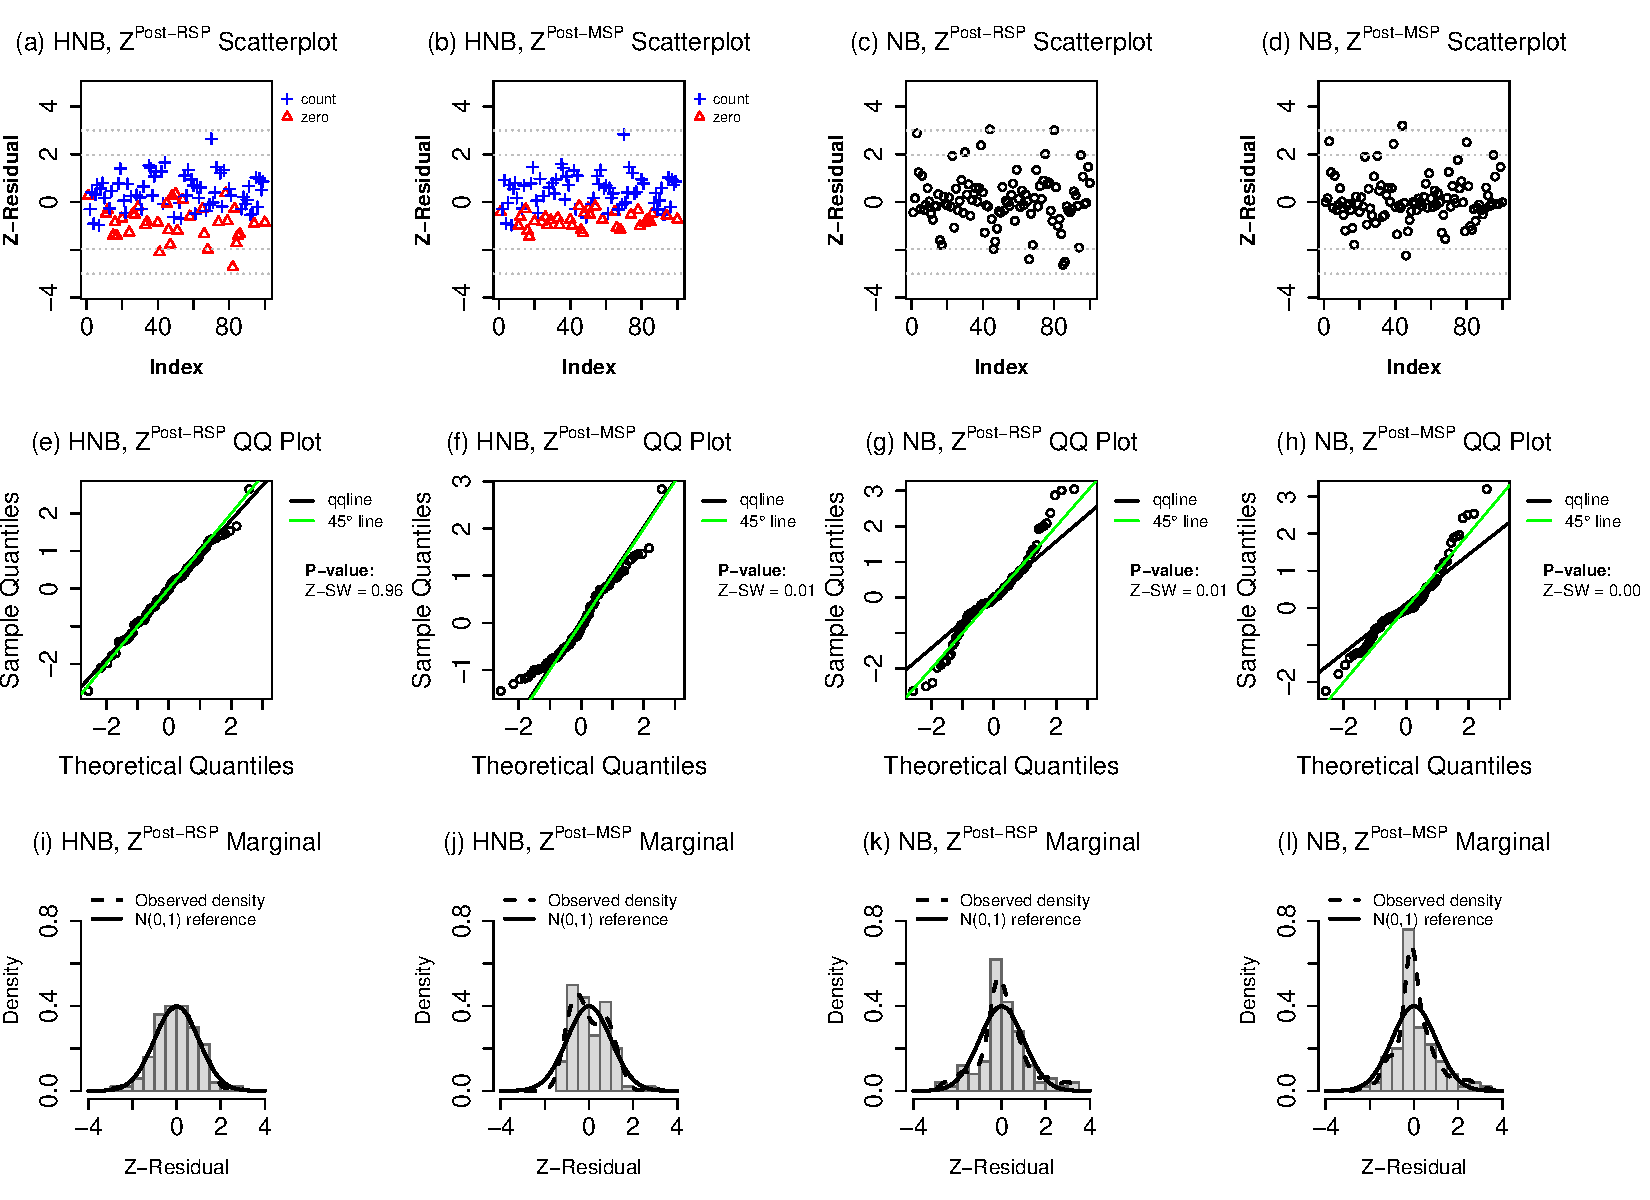
\includegraphics[width=\textwidth, height=\textwidth]{plot/sim1_overall_qq_scatter_plot2.pdf}
\caption{Visual diagnostics with posterior RSP and MSP Z-residuals for HNB and NB models. The first row displays residual-versus-index plots, with positive count observations and zero observations marked separately for the HNB fits. The second row presents QQ plots of the Z-residuals against the standard normal reference distribution, with Shapiro--Wilk $p$-values reported in the panels. The third row shows the marginal distributions of the Z-residuals, with histograms, empirical kernel densities, and the \(N(0,1)\) reference density overlaid.}
\label{fig_scatter_qq_sim1}

\end{figure}

To further evaluate the performance of all diagnostic tests introduced in Section~\ref{M-ZRESID}, we examine the empirical distributions of their $p$-values using replicated datasets, as displayed in Figure \ref{fig_histogram_sim1}. The histograms are based on 500 replications with a sample size of $n=100$ and a zero proportion $\mhu\approx 30\%$. For each diagnostic method, we show two distributions: a blue histogram representing the $p$-values when the true HNB model is fitted (the null hypothesis), and a red histogram showing the $p$-values when a misspecified NB model is fitted (the alternative hypothesis). A well-calibrated diagnostic test should produce a $p$-value distribution that is approximately uniform under the null hypothesis, while a powerful test should have a distribution heavily concentrated towards zero under the alternative hypothesis.

\begin{figure}[ht]
\centering
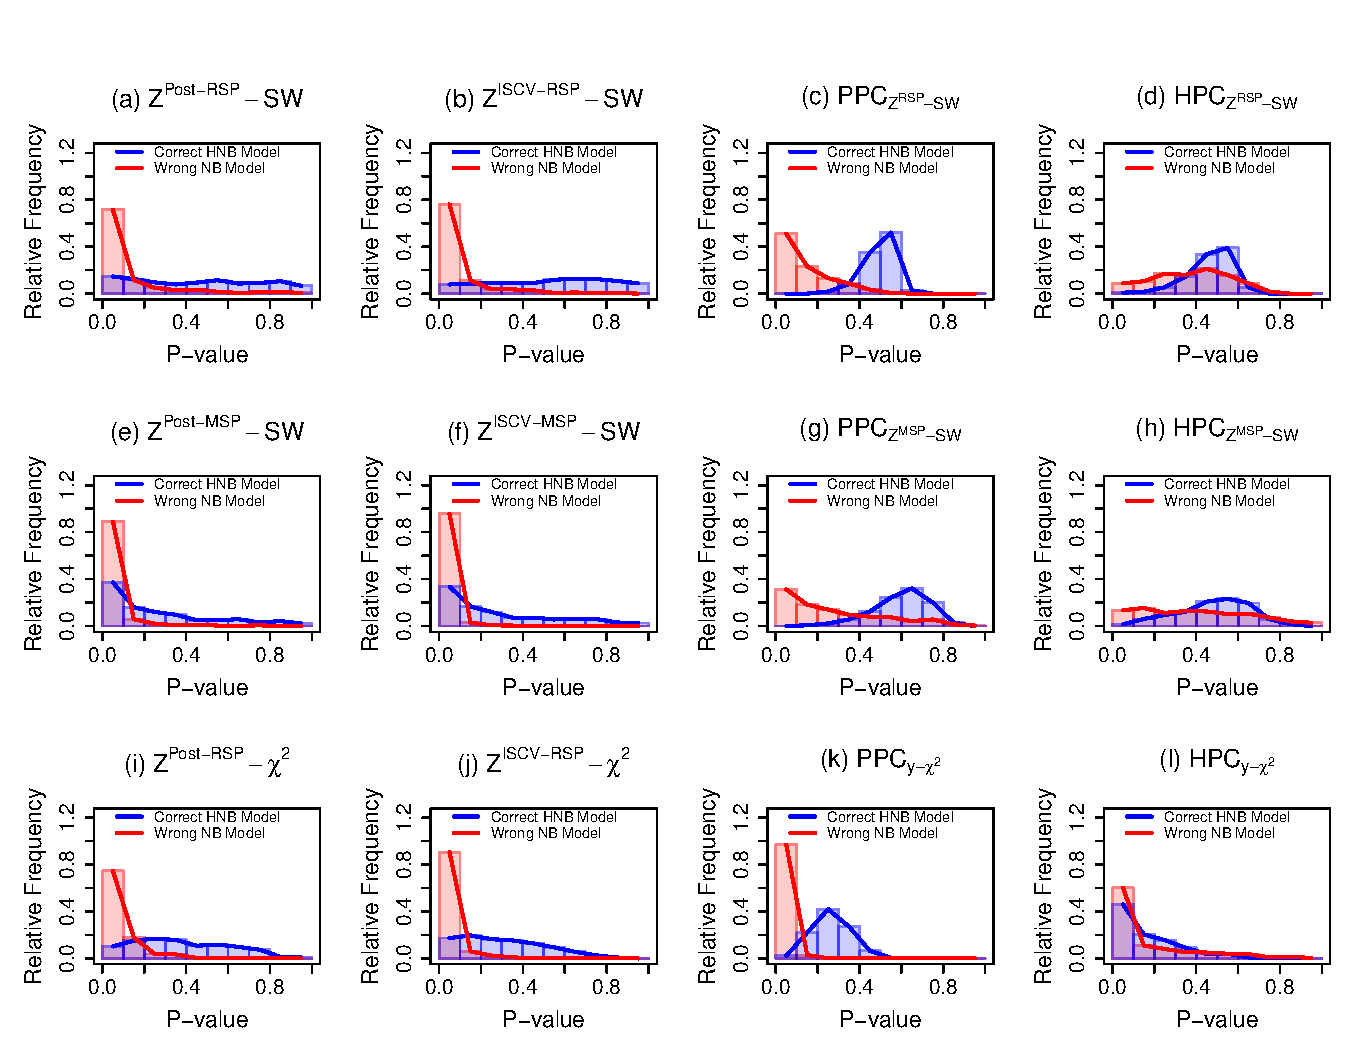
\includegraphics[width=\textwidth, height=0.8\textwidth]{plot/sim1_hnb_misdistr_histograms_n100.pdf}
\caption{Empirical distributions of $p$-values for various diagnostic methods under the true HNB model (blue histograms) and the wrong NB model (red histograms), based on 500 replications with sample size $n=100$ and zero proportion $\mhu\approx 30\%$.
}
\label{fig_histogram_sim1}
\end{figure}


We compare the $p$-value distributions from Z-residual diagnostics and posterior predictive checks and holdout predictive checks using similar parameter-wise tests. As shown in Figures \ref{fig_histogram_sim1}(a) and (b), the RSP-based Z-residual method with the SW test produces well-calibrated, uniform $p$-values distributions under the true model and exhibits high power under the wrong model, with $p$-values heavily concentrated near zero; in contrast, the PPC with the same SW test statistic (Figure \ref{fig_histogram_sim1}(c)) exhibits a severe conservative bias---with $p$-values concentrated around 0.5 under the true model---and has noticeably lower power under the misspecified NB model. The corresponding HPC check is also conservative and shows even weaker separation between the true HNB and wrong NB models (Figure \ref{fig_histogram_sim1}(d)). Similarly, Figures \ref{fig_histogram_sim1}(e) and (f) show that MSP-based posterior and ISCV Z-residual diagnostics can be poorly calibrated under the true discrete model, while Figures \ref{fig_histogram_sim1}(g) and (h) show that the corresponding PPC and HPC methods based on MSP Z-residuals are also highly conservative and significantly less powerful than the corresponding MSP-based Z-residual diagnostics. The $p$-values from a PPC with the $\chi^2$ statistic are also severely biased toward 0.5 under the true HNB model. However, this approach is highly powerful in this scenario and more powerful than the $\chi^2$ test applied to RSP-based posterior and ISCV Z-residuals (Figures \ref{fig_histogram_sim1}(i)--(k)). The corresponding HPC with the $y-\chi^2$ statistic is less stable, producing many small $p$-values even under the true HNB model in this sparse count setting (Figure \ref{fig_histogram_sim1}(l)). In summary, these results confirm the asymptotic findings in Section \ref{M-sec:asympZvsPPC}: tests based on RSP Z-residuals are asymptotically calibrated, whereas PPC methods are not, and HPC methods can lose power or become unstable depending on the statistic, although a PPC with a well-chosen test statistic ($\chi^2$ here) could achieve high power in some scenarios.

We also compare the performance of different types of Z-residual. The RSP Z-residuals (Figure \ref{fig_histogram_sim1} (a), (b), (i), and (j)) consistently produce $p$-value distributions that are approximately uniform under the true HNB model, indicating robust calibration regardless of whether the posterior or ISCV method is used, which confirms the asymptotic analysis in Section \ref{M-sec:asympZvsPPC}. Under the misspecified NB model (red histograms), their $p$-values are heavily concentrated towards zero, demonstrating high power. In contrast, the MSP Z-residuals methods (Figure \ref{fig_histogram_sim1} (d) and (e)) exhibit a clear lack of uniformity under the true model, with $p$-values biased towards larger values. More precisely, the MSP-based posterior and ISCV diagnostics are shown in Figures \ref{fig_histogram_sim1}(e) and (f), while the PPC and HPC versions based on MSP Z-residuals are shown in Figures \ref{fig_histogram_sim1}(g) and (h). Although these methods also show high power, their poor calibration under the null hypothesis makes them less reliable than their RSP counterparts.


\begin{figure}[htp]
\centering
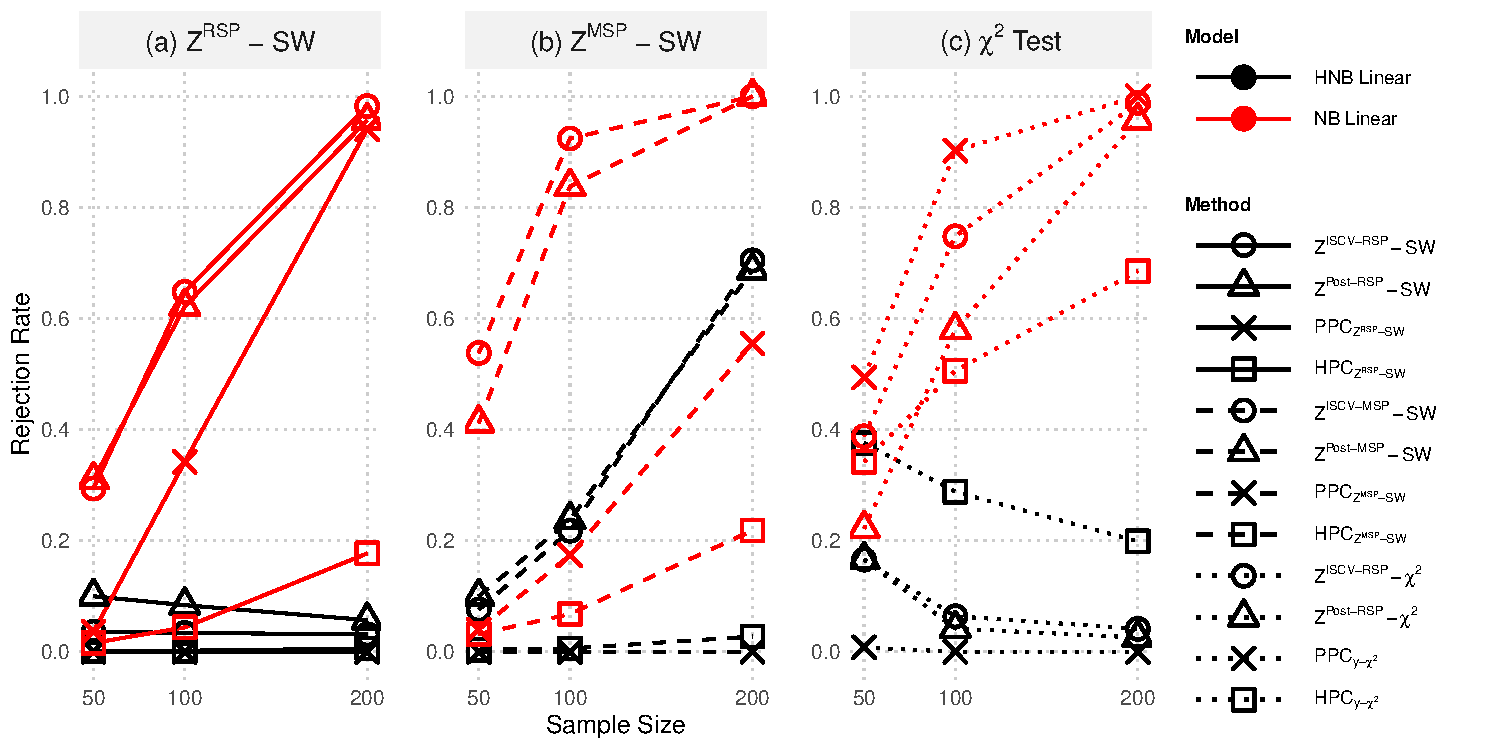
\includegraphics[width=1\textwidth, height=\textwidth]{plot/sim1_hnb_misdistr_rejection_rate_plot.pdf}
\caption{Empirical model rejection rates for various diagnostic methods under different sample sizes ($n=50, 100, 200$), based on 500 replications with a nominal significance level of 0.05. The rejection rates under the true HNB model (Type I error rates) are shown in black, and the rates under the wrong NB model (power) are shown in red.}
\label{fig_rejection_rate_sim1}
\end{figure}


\newcommand{\blankrate}{\rule{1.8em}{0.4pt}}
\begin{table}[!htbp]
\centering
\caption{Empirical rejection rates for the HNB versus NB wrong-family simulation. The nominal significance level is 0.05. Rejection rates under the correctly specified HNB model estimate type I error rates, whereas rejection rates under the misspecified NB model estimate power. Monte Carlo standard errors can be computed as $\sqrt{\hat p(1-\hat p)/R}$; with $R=500$, the Monte Carlo standard error is approximately 0.010 for a rejection rate near 0.05.}
\label{tab:supp_hnb_nb_rejection_rates}
\scriptsize
\setlength{\tabcolsep}{4pt}
\renewcommand{\arraystretch}{1.15}
\begin{tabular}{lrrrrrr}
\toprule
Method 
& \multicolumn{2}{c}{$n=50$} 
& \multicolumn{2}{c}{$n=100$} 
& \multicolumn{2}{c}{$n=200$} \\
\cmidrule(lr){2-3} \cmidrule(lr){4-5} \cmidrule(lr){6-7}
& HNB & NB 
& HNB & NB 
& HNB & NB \\
\midrule
$Z^{\mathrm{Post\mbox{-}RSP}}$--SW 
& 0.100 & 0.310 & 0.084 & 0.622 & 0.057 & 0.957 \\
$Z^{\mathrm{ISCV\mbox{-}RSP}}$--SW 
& 0.036 & 0.294 & 0.034 & 0.648 & 0.031 & 0.982 \\
PPC$_{Z^{\mathrm{RSP}}\text{--SW}}$ 
& $<0.001$  & 0.036 & $<0.001$  & 0.342 & $<0.001$  & 0.941 \\
HPC$_{Z^{\mathrm{RSP}}\text{--SW}}$ 
& 0.002 & 0.016 & 0.002 & 0.044 & 0.006 & 0.177 \\
\midrule
$Z^{\mathrm{Post\mbox{-}MSP}}$--SW 
& 0.100 & 0.412 & 0.238 & 0.838 & 0.687 & 1.000 \\
$Z^{\mathrm{ISCV\mbox{-}MSP}}$--SW 
& 0.076 & 0.538 & 0.218 & 0.924 & 0.705 & 1.000 \\
PPC$_{Z^{\mathrm{MSP}}\text{--SW}}$ 
& $<0.001$  & 0.040 & $<0.001$  & 0.174 & $<0.001$  & 0.555 \\
HPC$_{Z^{\mathrm{MSP}}\text{--SW}}$ 
& 0.004 & 0.032 & 0.006 & 0.068 & 0.028 & 0.219 \\
\midrule
$Z^{\mathrm{Post\mbox{-}RSP}}$--$\chi^2$ 
& 0.166 & 0.222 & 0.042 & 0.580 & 0.026 & 0.957 \\
$Z^{\mathrm{ISCV\mbox{-}RSP}}$--$\chi^2$ 
& 0.166 & 0.388 & 0.064 & 0.748 & 0.041 & 0.988 \\
PPC$_{y\text{--}\chi^2}$ 
& 0.008 & 0.494 & $<0.001$  & 0.902 & $<0.001$  & 1.000 \\
HPC$_{y\text{--}\chi^2}$ 
& 0.376 & 0.342 & 0.288 & 0.506 & 0.199 & 0.685 \\
\bottomrule
\end{tabular}

\vspace{1mm}
\begin{minipage}{0.95\textwidth}
\footnotesize
\textit{Note.} HNB denotes the correctly specified hurdle negative binomial model,
and NB denotes the misspecified negative binomial model. SW denotes the
Shapiro--Wilk normality test, and $\chi^2$ denotes the omnibus chi-square test.
HPC denotes holdout predictive checks.
\end{minipage}
\end{table}

Finally, we assess model rejection rates for different sample sizes ($n=50, 100, 200$), with results broken down by test statistic in Figure \ref{fig_rejection_rate_sim1}. An ideal test should maintain a Type I error rate near 0.05 under the true model while having high power (rejection rate near 1) under a misspecified model. Figure \ref{fig_rejection_rate_sim1}(a) shows that when using an SW test on RSP Z-residuals, both the posterior and ISCV approaches maintain Type I error rates close to the nominal 0.05 level, demonstrating robust calibration across all sample sizes. In contrast, the corresponding PPC is overly conservative, with Type I error rates near zero and significantly lower power (e.g., $\sim 0.036$ ($-\!\times\!-$) vs. $\sim 0.310$ ($-\!\triangle\!-$) for $n=50$) (Table \ref{tab:supp_hnb_nb_rejection_rates}). The corresponding HPC check is also conservative and has even lower power, especially for small and moderate sample sizes. Under the wrong model, the posterior and ISCV RSP Z-residual SW tests show increasing power, with rejection rates approaching 1 as $n$ reaches 200, whereas the PPC improves more slowly and the HPC remains much less powerful.

Figure \ref{fig_rejection_rate_sim1}(b) presents the results for MSP-based methods. SW tests applied to MSP Z-residuals (both posterior and ISCV) are poorly calibrated, showing unacceptably high Type I error rates under the true model. Despite their high power, this makes them unreliable for formal hypothesis testing. The corresponding PPC and HPC methods are again overly conservative and have very low power.

Figure \ref{fig_rejection_rate_sim1}(c) illustrates the methods using a $\chi^2$ statistic. The $\chi^2$ tests based on RSP-based Z-residuals (both posterior and ISCV) maintain Type I error rates close to the nominal 0.05 level for larger sample sizes, although some finite-sample deviation is visible at $n=50$. This contrasts with the PPC with a $\chi^2$ statistic, which is conservatively biased with a Type I error rate near zero, although it achieves the highest power in these scenarios. In contrast, the corresponding HPC with the $\chi^2$ statistic is unstable in this sparse count setting, showing inflated rejection rates even under the correctly specified HNB model; therefore, its apparent power should be interpreted cautiously. The corresponding numerical rejection rates are reported in Table~\ref{tab:supp_hnb_nb_rejection_rates}.

\clearpage

\subsection{Diagnostics for Mixed Misspecifications in Response Family and Covariate Functional Form Using the Synthetic Dataset from \S\ref{M-sec:sim-nl}}
\label{sec:sens_family_function}

To demonstrate how a joint analysis of graphical and numerical Z-residual diagnostics can disentangle multiple sources of model deficiency, we conducted an additional simulation study using the synthetic dataset ($n=50$) introduced in Figure~\ref{M-fig_scatter_boxplot_sim2} of the main text. Four fitted models were compared, representing all combinations of correct and misspecified components: HNB-log (fully correct), HNB-linear (misspecified functional form), NB-log (misspecified response family), and NB-linear (misspecified in both). 

\begin{figure}[!htbp]
\centering

\includegraphics[width=\textwidth]{plot/sim2_NB_model_scatter_box_plot.png}
\caption{Posterior RSP Z-residual diagnostics for the NB models fitted to the HNB-generated dataset from Section~\ref{M-sec:sim-nl} of the main text. Panels (a) and (b) display the NB-log model, which misspecifies the response family while maintaining the correct logarithmic functional form for $X_1$. Panels (c) and (d) illustrate the NB-linear model, which misspecifies both the response family and the functional form of $X_1$. Scatterplots plot posterior RSP Z-residuals against $X_1$, with triangles denoting zero-count observations; boxplots group the residuals across $X_1$ intervals.}
\label{fig:sens_nb_residual_x1}
\end{figure}

Visual diagnostics reveal the distinct consequences of each misspecification type and guide subsequent model refinement. Figure~\ref{fig:sens_nb_residual_x1} presents the residual-versus-$X_1$ scatterplots and grouped boxplots for the two NB models. For the NB-log model (panels a and b), the Z-residual LOWESS curve exhibits a nearly linear upward trend with respect to $X_1$. This trend has a clear statistical interpretation: in the true HNB process, the hurdle component causes the probability of a positive count to increase with $X_1$. Fitting a single NB family forces this increasing probability into the NB mean structure, necessitating an additional linear term in $X_1$ beyond the specified $\log X_1$ effect. The observed residual trend accurately isolates this missing component. Furthermore, the Z-residuals of the zero counts (triangles) are distinctly separated from those of the positive counts. This divergence indicates that the NB family fails to capture the excess zeros, directly motivating a zero-modified specification such as the hurdle NB. The NB-linear model (panels c and d) inherits these family-related deficiencies while additionally displaying a pronounced curvature in the mean trend, alongside location shifts across $X_1$ intervals. These features reflect the increased severity of the functional-form error.

\begin{table}[!htbp]
\centering
\caption{Z-residual diagnostic $p$-values for the response-family sensitivity analysis, using the HNB-generated dataset from Section~\ref{M-sec:sim-nl} of the main text. The HNB-log and HNB-linear models were evaluated in the main text; the NB-log and NB-linear models are introduced here to assess response-family misspecification. Because the response is discrete and RSP Z-residuals depend on auxiliary randomization, we report median upper-bound $p$-values~(Eq.~\eqref{M-eqn:uppvalue-median}) for the posterior and ISCV RSP Z-residual tests. The AOV and Bartlett (BL) tests are evaluated against $X_1$. The logarithmic form is marked "Wrong" for the NB family because the $X_1$-dependent hurdle probability is improperly absorbed into the NB mean structure (see text).}
\label{tab:sens_family_function}
\scriptsize
\resizebox{\textwidth}{!}{%
\begin{tabular}{lllrrrrrrrr}
\toprule
 & & & \multicolumn{4}{c}{Posterior RSP Z-residuals} & \multicolumn{4}{c}{ISCV RSP Z-residuals} \\
\cmidrule(lr){4-7} \cmidrule(lr){8-11}
Model & Family & Functional form 
& SW & AOV-$X_1$ & BL-$X_1$ & $\chi^2$
& SW & AOV-$X_1$ & BL-$X_1$ & $\chi^2$ \\
\midrule
HNB-log    
& HNB (True) & log (True)   
& 0.904 & 0.630 & 0.120 & 0.884 
& 0.595 & 0.767 & 0.089 & 0.606 \\

HNB-linear 
& HNB (True) & linear (Wrong) 
& 0.282 & $<0.001$  & 0.002 & 0.165 
& 0.700 & $<0.001$  & 0.017 & 0.140 \\

NB-log     
& NB (Wrong) & log (Wrong)   
& 0.003 & 0.137 & 0.001 & 0.363 
& 0.044 & 0.281 & 0.001 & 0.178 \\

NB-linear  
& NB (Wrong) & linear (Wrong)
& $<0.001$  & 0.007 & $<0.001$  & 0.415 
& $<0.001$  & 0.004 & $<0.001$  & 0.368 \\
\bottomrule
\end{tabular}%
}
\end{table}

\begin{figure}[!htbp]
\centering
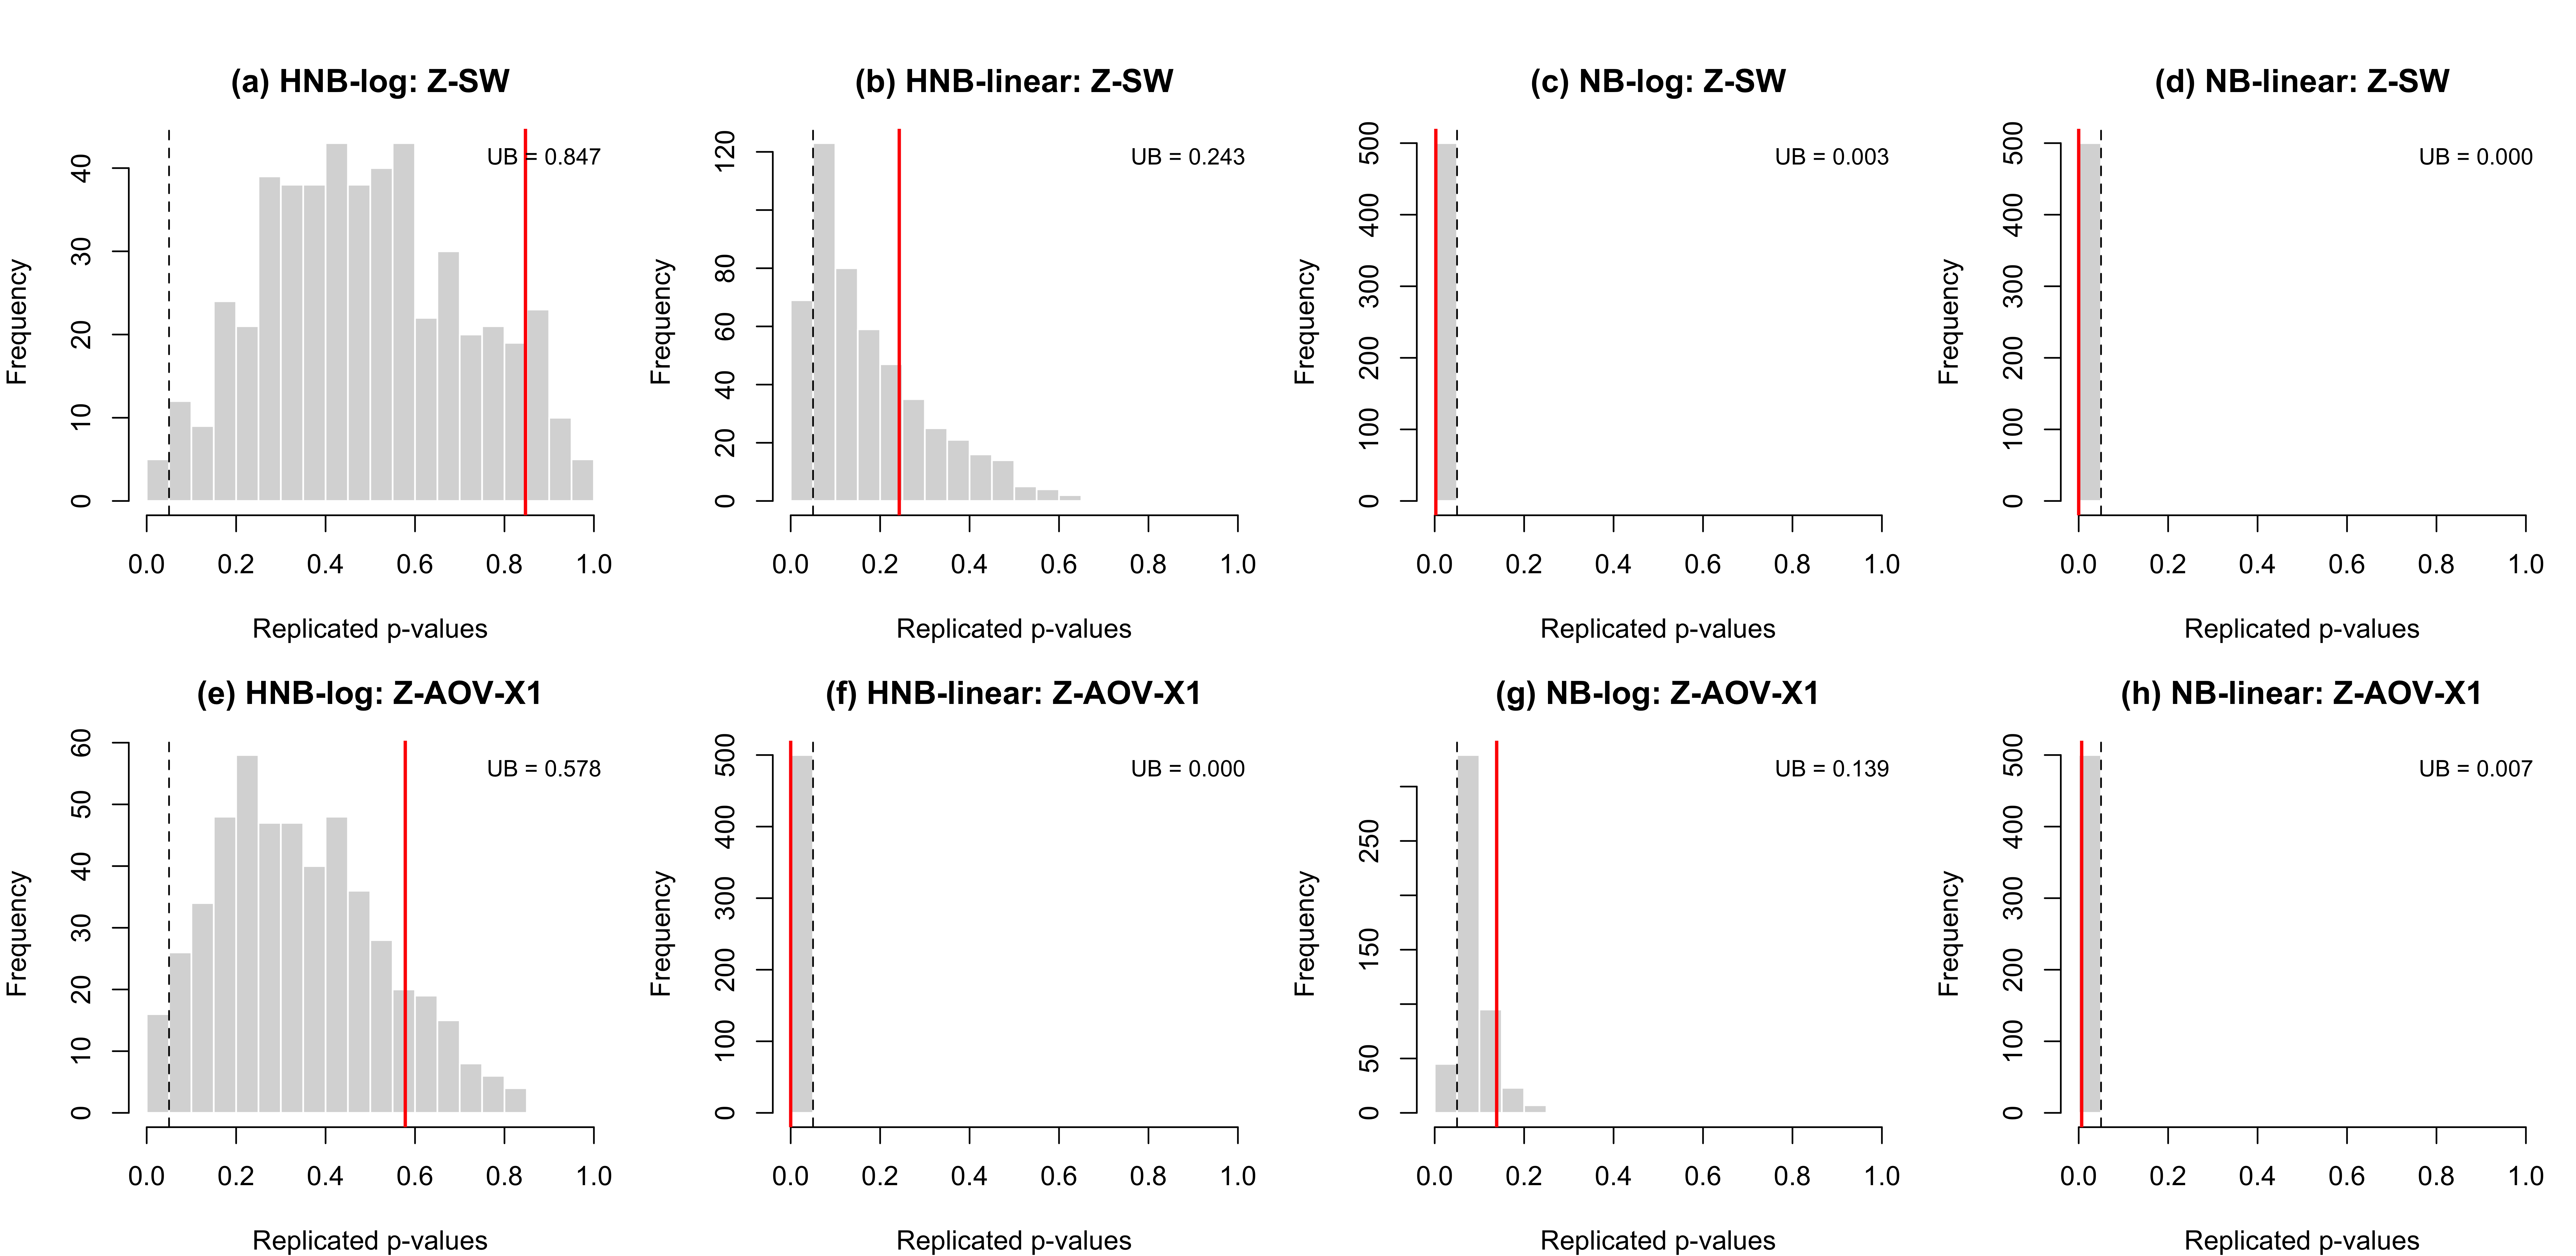
\includegraphics[width=\textwidth]{plot/sim2_replicated-z-pvalue-histograms.png}
\caption{Histograms of 500 replicated Z-residual test $p$-values for the four fitted models. These were obtained by re-randomizing the auxiliary uniform variables, $\bU$, used to construct the RSPs for the discrete response. The top row presents the SW tests, and the bottom row displays the AOV tests against $X_1$. Red vertical lines denote the corresponding median upper-bound $p$-values~(Eq.~\eqref{M-eqn:uppvalue-median}) from Table~\ref{tab:sens_family_function}, and dashed vertical lines indicate the $0.05$ significance level.}
\label{fig:sens_replicated_pvalue_hist}
\end{figure}

Numerical diagnostics corroborate and refine these visual findings. Figure~\ref{fig:sens_replicated_pvalue_hist} displays the distributions of the 500 replicated $p$-values, which are summarized in Table~\ref{tab:sens_family_function} via their median upper bounds. For the correctly specified HNB-log model, all tests appropriately fail to reject the null hypothesis. Conversely, for the HNB-linear model, the overall SW test is non-significant, but the AOV test against $X_1$ strongly rejects the model, effectively isolating the localized functional-form error.

The NB-log model illustrates the consequences of an incorrect response family. The SW and Bartlett tests strongly reject the model, reflecting a fundamental distributional mismatch. The AOV test against $X_1$ yields larger median upper-bound $p$-values ($0.137$ and $0.281$). However, two considerations caution against interpreting these values as evidence of an adequate functional form. First, the upper-bound $p$-value~(Eq.~\eqref{M-eqn:uppvalue-median}) is inherently conservative: the replicated $p$-values for this test (Figure~\ref{fig:sens_replicated_pvalue_hist}g) concentrate within the $(0.05, 0.1)$ interval, revealing non-negligible evidence of a residual mean pattern against $X_1$ (as an aside, in supplementary simulations with other datasets, this upper-bound $p$-value frequently drops below $0.05$). Second, this residual mean pattern is theoretically expected under the true data-generating process. Because the hurdle component in the HNB process causes the probability of a positive count to increase with $X_1$, fitting a single NB family absorbs this dynamic into the NB mean structure. Consequently, the log-linear form alone fails to correctly specify the conditional mean. The moderate AOV signal thus represents a valid, albeit attenuated, detection of this induced mean distortion rather than a false alarm. This interpretation is corroborated by the near-linear residual trend in Figure~\ref{fig:sens_nb_residual_x1}a. Finally, the NB-linear model is decisively rejected by both the SW and AOV tests, simultaneously flagging the overall distributional failure and the severe functional-form error.

In summary, a joint evaluation of these diagnostics allows practitioners to better pinpoint a model's deficiencies, even though isolating the exact source of misspecification remains challenging. The overall SW test is highly sensitive to response-family misspecifications that alter the global residual distribution, while residual-versus-covariate scatterplots and grouped AOV tests are tuned to localized covariate functional-form errors. These two error sources are not entirely separable, however. As demonstrated by the NB-log example, a misspecified response family can itself distort the implied mean structure, causing family errors to legitimately propagate into covariate-specific tests. Given these interactions, a robust diagnostic workflow must combine multiple graphical and numerical residual diagnostics, supplemented by model comparison metrics such as information criteria. Developing Z-residual tests and visualization methods that offer both high sensitivity and specificity to particular forms of model misspecification remains a crucial direction for future research. The versatility of Z-residuals provides a strong foundation for this ongoing effort.

\clearpage

\subsection{Tabular Rejection Rates of Main-text Simulations}

To make the empirical type I error and power explicit, Tables~\ref{tab:supp_ig_rejection_rates} and \ref{tab:supp_hnb_nonlinear_rejection_rates} detail the numerical rejection rates corresponding to Figures~\ref{M-fig_rejection_rate_ig} and~\ref{M-fig_rejection_rate_sim2}. Based on $R=500$ replications, Monte Carlo standard errors ($\sqrt{\hat p(1-\hat p)/R}$) range from roughly 0.010 (95\% margin of error $\approx 0.019$) at a 0.05 rejection rate, up to 0.022 (margin of error $\approx 0.044$) at a 0.50 rejection rate.

\begin{table}[!htbp]
\centering
\caption{Rejection rates ($\alpha=0.05$) for the continuous IG simulation (Section~\ref{M-sec:simulation_piecewise_ig}), showing type I error (``Correct'' piecewise model) and power (``Wrong'' linear model). Tests: Shapiro--Wilk (SW), grouped ANOVA (AOV-$X_1$), and omnibus chi-square ($\chi^2$).}
\label{tab:supp_ig_rejection_rates}
\scriptsize
\setlength{\tabcolsep}{4pt}
\renewcommand{\arraystretch}{1.15}
\begin{tabular}{lrrrrrr}
\toprule
Method 
& \multicolumn{2}{c}{$n=50$} 
& \multicolumn{2}{c}{$n=100$} 
& \multicolumn{2}{c}{$n=200$} \\
\cmidrule(lr){2-3} \cmidrule(lr){4-5} \cmidrule(lr){6-7}
& Correct & Wrong 
& Correct & Wrong 
& Correct & Wrong \\
\midrule
$Z^{\mathrm{Post\mbox{-}RSP}}$--SW 
& 0.046 & 0.034 & 0.020 & 0.080 & 0.036 & 0.092 \\
$Z^{\mathrm{ISCV\mbox{-}RSP}}$--SW 
& 0.068 & 0.056 & 0.040 & 0.093 & 0.052 & 0.128 \\
PPC$_{Z^{\mathrm{RSP}}\text{--SW}}$ 
& $<0.001$  & 0.002 & $<0.001$  & 0.007 & 0.008 & 0.074 \\
HPC$_{Z^{\mathrm{RSP}}\text{--SW}}$ 
& $<0.001$  & $<0.001$  & 0.007 & $<0.001$  & 0.022 & 0.028 \\
\midrule
$Z^{\mathrm{Post\mbox{-}RSP}}$--AOV-$X_1$ 
& 0.028 & 0.420 & 0.020 & 0.873 & 0.022 & 1.000 \\
$Z^{\mathrm{ISCV\mbox{-}RSP}}$--AOV-$X_1$ 
& 0.024 & 0.412 & 0.020 & 0.880 & 0.022 & 1.000 \\
PPC$_{Z^{\mathrm{RSP}}\text{--AOV-}X_1}$ 
& 0.010 & 0.276 & 0.020 & 0.813 & 0.034 & 1.000 \\
HPC$_{Z^{\mathrm{RSP}}\text{--AOV-}X_1}$ 
& 0.015 & 0.032 & 0.020 & 0.087 & 0.036 & 0.410 \\
\midrule
$Z^{\mathrm{Post\mbox{-}RSP}}$--$\chi^2$ 
& 0.002 & $<0.001$  & $<0.001$  & $<0.001$  & $<0.001$  & $<0.001$  \\
$Z^{\mathrm{ISCV\mbox{-}RSP}}$--$\chi^2$ 
& 0.002 & $<0.001$  & $<0.001$  & $<0.001$  & $<0.001$  & $<0.001$  \\
PPC$_{y\text{--}\chi^2}$ 
& $<0.001$  & $<0.001$  & $<0.001$  & $<0.001$  & $<0.001$  & $<0.001$  \\
HPC$_{y\text{--}\chi^2}$ 
& 0.088 & 0.128 & 0.120 & 0.100 & 0.088 & 0.126 \\
\bottomrule
\end{tabular}
\end{table}

\begin{table}[!htbp]
\centering
\caption{Rejection rates ($\alpha=0.05$) for the nonlinear HNB simulation (Section~\ref{M-sec:sim-nl}), showing type I error (``Correct'' logarithmic model) and power (``Wrong'' linear model). Test abbreviations follow Table~\ref{tab:supp_ig_rejection_rates}.}
\label{tab:supp_hnb_nonlinear_rejection_rates}
\scriptsize
\setlength{\tabcolsep}{4pt}
\renewcommand{\arraystretch}{1.15}
\begin{tabular}{lrrrrrr}
\toprule
Method 
& \multicolumn{2}{c}{$n=50$} 
& \multicolumn{2}{c}{$n=100$} 
& \multicolumn{2}{c}{$n=200$} \\
\cmidrule(lr){2-3} \cmidrule(lr){4-5} \cmidrule(lr){6-7}
& Correct & Wrong 
& Correct & Wrong 
& Correct & Wrong \\
\midrule
$Z^{\mathrm{Post\mbox{-}RSP}}$--SW 
& 0.130 & 0.390 & 0.072 & 0.602 & 0.050 & 0.862 \\
$Z^{\mathrm{ISCV\mbox{-}RSP}}$--SW 
& 0.084 & 0.140 & 0.062 & 0.326 & 0.046 & 0.668 \\
PPC$_{Z^{\mathrm{RSP}}\text{--SW}}$ 
& $<0.001$  & $<0.001$  & $<0.001$  & 0.038 & 0.004 & 0.366 \\
HPC$_{Z^{\mathrm{RSP}}\text{--SW}}$ 
& $<0.001$  & 0.002 & 0.002 & $<0.001$  & 0.004 & 0.004 \\
\midrule
$Z^{\mathrm{Post\mbox{-}RSP}}$--AOV-$X_1$ 
& 0.032 & 0.906 & 0.028 & 1.000 & 0.030 & 1.000 \\
$Z^{\mathrm{ISCV\mbox{-}RSP}}$--AOV-$X_1$ 
& 0.032 & 0.846 & 0.024 & 1.000 & 0.032 & 1.000 \\
PPC$_{Z^{\mathrm{RSP}}\text{--AOV-}X_1}$ 
& $<0.001$  & 0.826 & 0.008 & 1.000 & 0.012 & 1.000 \\
HPC$_{Z^{\mathrm{RSP}}\text{--AOV-}X_1}$ 
& 0.011 & 0.021 & 0.010 & 0.244 & 0.012 & 0.862 \\
\midrule
$Z^{\mathrm{Post\mbox{-}RSP}}$--$\chi^2$ 
& 0.060 & 0.206 & 0.010 & 0.172 & 0.002 & 0.252 \\
$Z^{\mathrm{ISCV\mbox{-}RSP}}$--$\chi^2$ 
& 0.096 & 0.264 & 0.028 & 0.300 & 0.018 & 0.418 \\
PPC$_{y\text{--}\chi^2}$ 
& 0.004 & $<0.001$  & 0.010 & $<0.001$  & 0.012 & $<0.001$  \\
HPC$_{y\text{--}\chi^2}$ 
& 0.352 & 0.230 & 0.224 & 0.070 & 0.160 & 0.024 \\
\bottomrule
\end{tabular}
\end{table}

\clearpage

\section{\textred{Additional Results of the Dolphin-sighting Data}}

\subsection{Posterior Summaries for the Selected Nonlinear HNB Model}\label{supp:add-tables}
\begin{table}[htbp]
\centering
\caption{Regression coefficients for the selected nonlinear HNB model fitted to the dolphin-sighting data. Columns report posterior mean (Estimate), Monte Carlo SE (Est.Error), 95\% credible interval, and $\hat R$.}
\label{tab:reg_coefs}
\begin{tabular}{lrrrrr}
\toprule
 & \multicolumn{1}{c}{Estimate} & \multicolumn{1}{c}{Est.Error} & \multicolumn{1}{c}{l-95\% CI} & \multicolumn{1}{c}{u-95\% CI} & \multicolumn{1}{c}{$\hat{R}$} \\
\midrule
Intercept      &  9.16  & 6.61 & -3.55 & 22.14 & 1.00 \\
hu\_Intercept  & -11.25 & 6.62 & -24.35 &  1.81 & 1.00 \\
below7.95      & -0.00  & 0.02 & -0.05 &  0.04 & 1.00 \\
above7.95      & -0.00  & 0.01 & -0.02 &  0.02 & 1.00 \\
temp           & -0.37  & 0.13 & -0.63 & -0.13 & 1.00 \\
dr             &  0.00  & 0.03 & -0.05 &  0.05 & 1.00 \\
salinity       &  0.08  & 0.19 & -0.30 &  0.45 & 1.00 \\
turbidity      &  0.14  & 0.13 & -0.11 &  0.39 & 1.00 \\
year2          & -0.52  & 0.41 & -1.33 &  0.29 & 1.00 \\
year3          &  0.34  & 0.34 & -0.33 &  0.99 & 1.00 \\
year4          &  1.98  & 1.49 & -0.83 &  5.06 & 1.00 \\
year5          &  0.43  & 0.66 & -0.84 &  1.74 & 1.00 \\
year6          & -1.60  & 0.54 & -2.65 & -0.55 & 1.00 \\
hu\_below7.95  &  0.12  & 0.02 &  0.08 &  0.16 & 1.00 \\
hu\_above7.95  &  0.03  & 0.01 &  0.01 &  0.05 & 1.00 \\
hu\_temp       & -0.16  & 0.12 & -0.39 &  0.08 & 1.00 \\
hu\_dr         &  0.01  & 0.02 & -0.04 &  0.06 & 1.00 \\
hu\_salinity   &  0.54  & 0.19 &  0.18 &  0.92 & 1.00 \\
hu\_turbidity  &  0.03  & 0.13 & -0.23 &  0.29 & 1.00 \\
hu\_year2      & -1.41  & 0.39 & -2.17 & -0.65 & 1.00 \\
hu\_year3      & -0.37  & 0.33 & -1.03 &  0.28 & 1.00 \\
hu\_year4      &  3.24  & 1.39 &  0.72 &  6.19 & 1.00 \\
hu\_year5      &  0.89  & 0.62 & -0.33 &  2.09 & 1.00 \\
hu\_year6      & -2.29  & 0.50 & -3.29 & -1.31 & 1.00 \\
\bottomrule
\end{tabular}
\end{table}

\clearpage

\subsection{Prior Sensitivity Analysis}\label{prior_analysis}

Because Z-residuals are constructed from posterior or cross-validatory predictive distributions, the resulting diagnostics may depend on the prior specification, especially when the prior is informative or the sample size is small. We therefore conducted a prior sensitivity analysis for the dolphin-sighting data.

We compared three prior specifications: the baseline prior used in the main analysis, a tighter prior, and a more diffuse prior. The tight setting used smaller prior standard deviations for regression coefficients and intercepts, while the diffuse setting used larger prior standard deviations. The three prior specifications are summarized in Table~\ref{tab:prior_sensitivity_specs}. 

\begin{table}[!htbp] 
\centering 
\caption{Prior specifications used in the prior sensitivity analysis for the dolphin-sighting data. Gamma priors use the shape-rate parameterization.} 
\label{tab:prior_sensitivity_specs} 
\small 
\setlength{\tabcolsep}{6pt} 
\renewcommand{\arraystretch}{1.15} 
\begin{tabular}{lccc} 
\toprule 
Prior component & Baseline & Tight & Diffuse \\ 
\midrule 
Regression coefficients 
& $\mathrm{Normal}(0,2)$ 
& $\mathrm{Normal}(0,1)$ 
& $\mathrm{Normal}(0,5)$ \\ 
Intercepts 
& $\mathrm{Normal}(0,5)$ 
& $\mathrm{Normal}(0,2.5)$ 
& $\mathrm{Normal}(0,10)$ \\ 
Dispersion/shape parameter 
& $\mathrm{Gamma}(2,0.5)$ 
& $\mathrm{Gamma}(4,1)$ 
& $\mathrm{Gamma}(2,0.1)$ \\ 
\bottomrule 
\end{tabular} 
\end{table}

Figure~\ref{fig_prior_sensitivity} shows the diagnostic $p$-values under the three prior specifications for the linear HNB, linear NB, nonlinear HNB, and nonlinear NB models. Overall, the diagnostic conclusions are qualitatively stable across the prior choices. The AOV diagnostic against depth continues to give small $p$-values for the linear HNB and NB models, indicating remaining nonlinear structure in depth, whereas the corresponding $p$-values are large for the nonlinear HNB and NB models. The Shapiro--Wilk and \(\chi^2\)-type diagnostics also show similar qualitative patterns across the three prior settings. These results suggest that the main real-data conclusions are not driven by the particular baseline prior specification.
\begin{figure}[htp] 
\centering 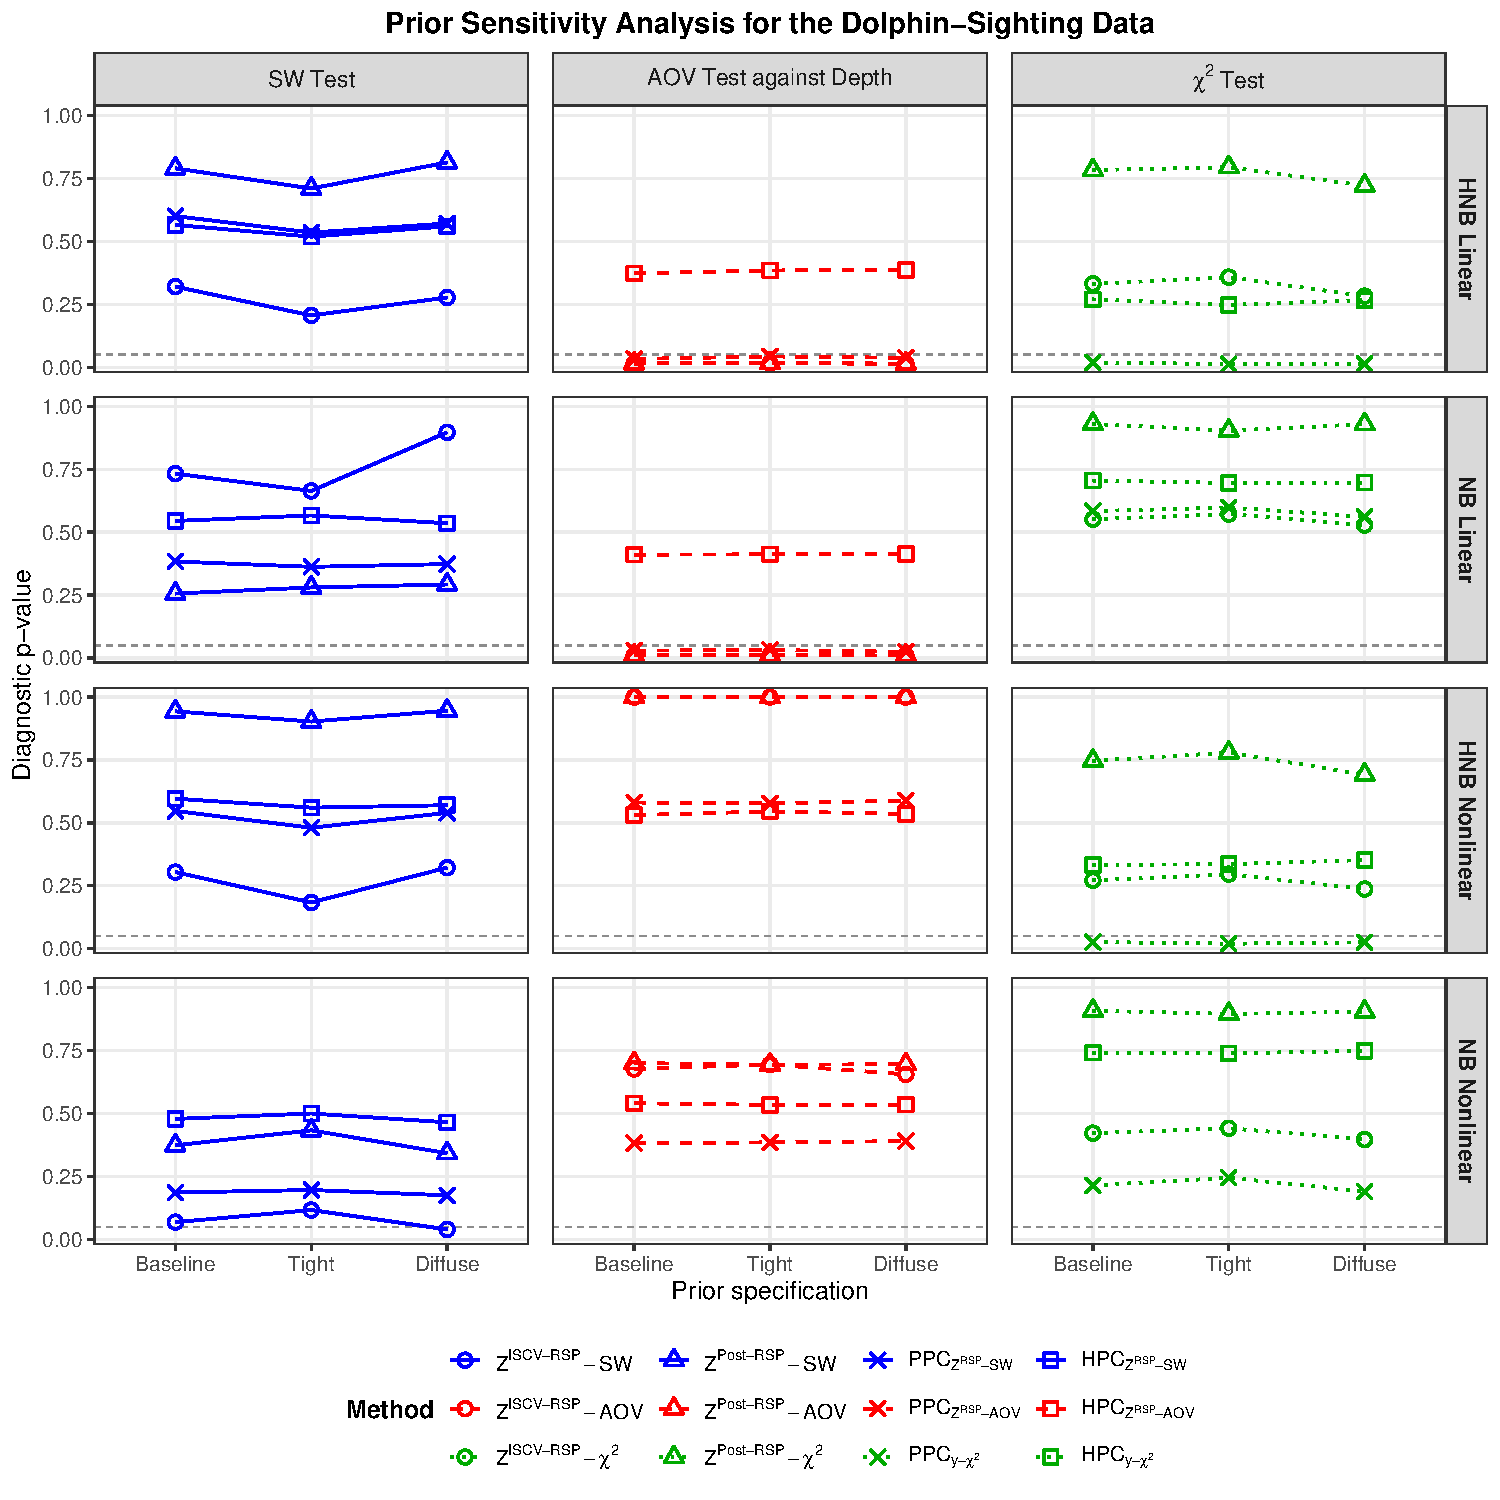
\includegraphics[width=\textwidth, height=\textwidth]{plot/appendix_prior_sensitivity_all_methods.pdf} \caption{Prior sensitivity analysis for the dolphin-sighting data. Diagnostic $p$-values are shown for the linear HNB, linear NB, nonlinear HNB, and nonlinear NB models under three prior specifications: baseline, tight, and diffuse. Columns correspond to the Shapiro--Wilk test, the ANOVA test against depth, and the omnibus chi-square test. The horizontal dashed line marks the nominal 0.05 level. The qualitative diagnostic conclusions are stable across the three prior specifications: the ANOVA diagnostic continues to reject the linear HNB and NB models, while the nonlinear models are not rejected by the ANOVA diagnostic.} 
\label{fig_prior_sensitivity} 
\end{figure}

\clearpage


\subsection{Sensitivity of the Z-AOV Test to the Number of Groups}\label{sec:aov_bin_analysis}

Figure~\ref{fig_binning_sensitivity} examines the sensitivity of the Z-AOV diagnostic to the number of  intervals ($k$) of the variable \texttt{depth}. We recreated the grouped boxplots and AOV tests using $k \in \{5,10,15,20\}$ equally spaced intervals. To account for the discrete response, we repeated the auxiliary randomization $J=500$ times for each $k$, summarizing the resulting $p$-values via the conservative upper-bound $p$-value for the median (Eq.~\ref{M-eqn:uppvalue-median}).


\begin{figure}[htp]
\centering
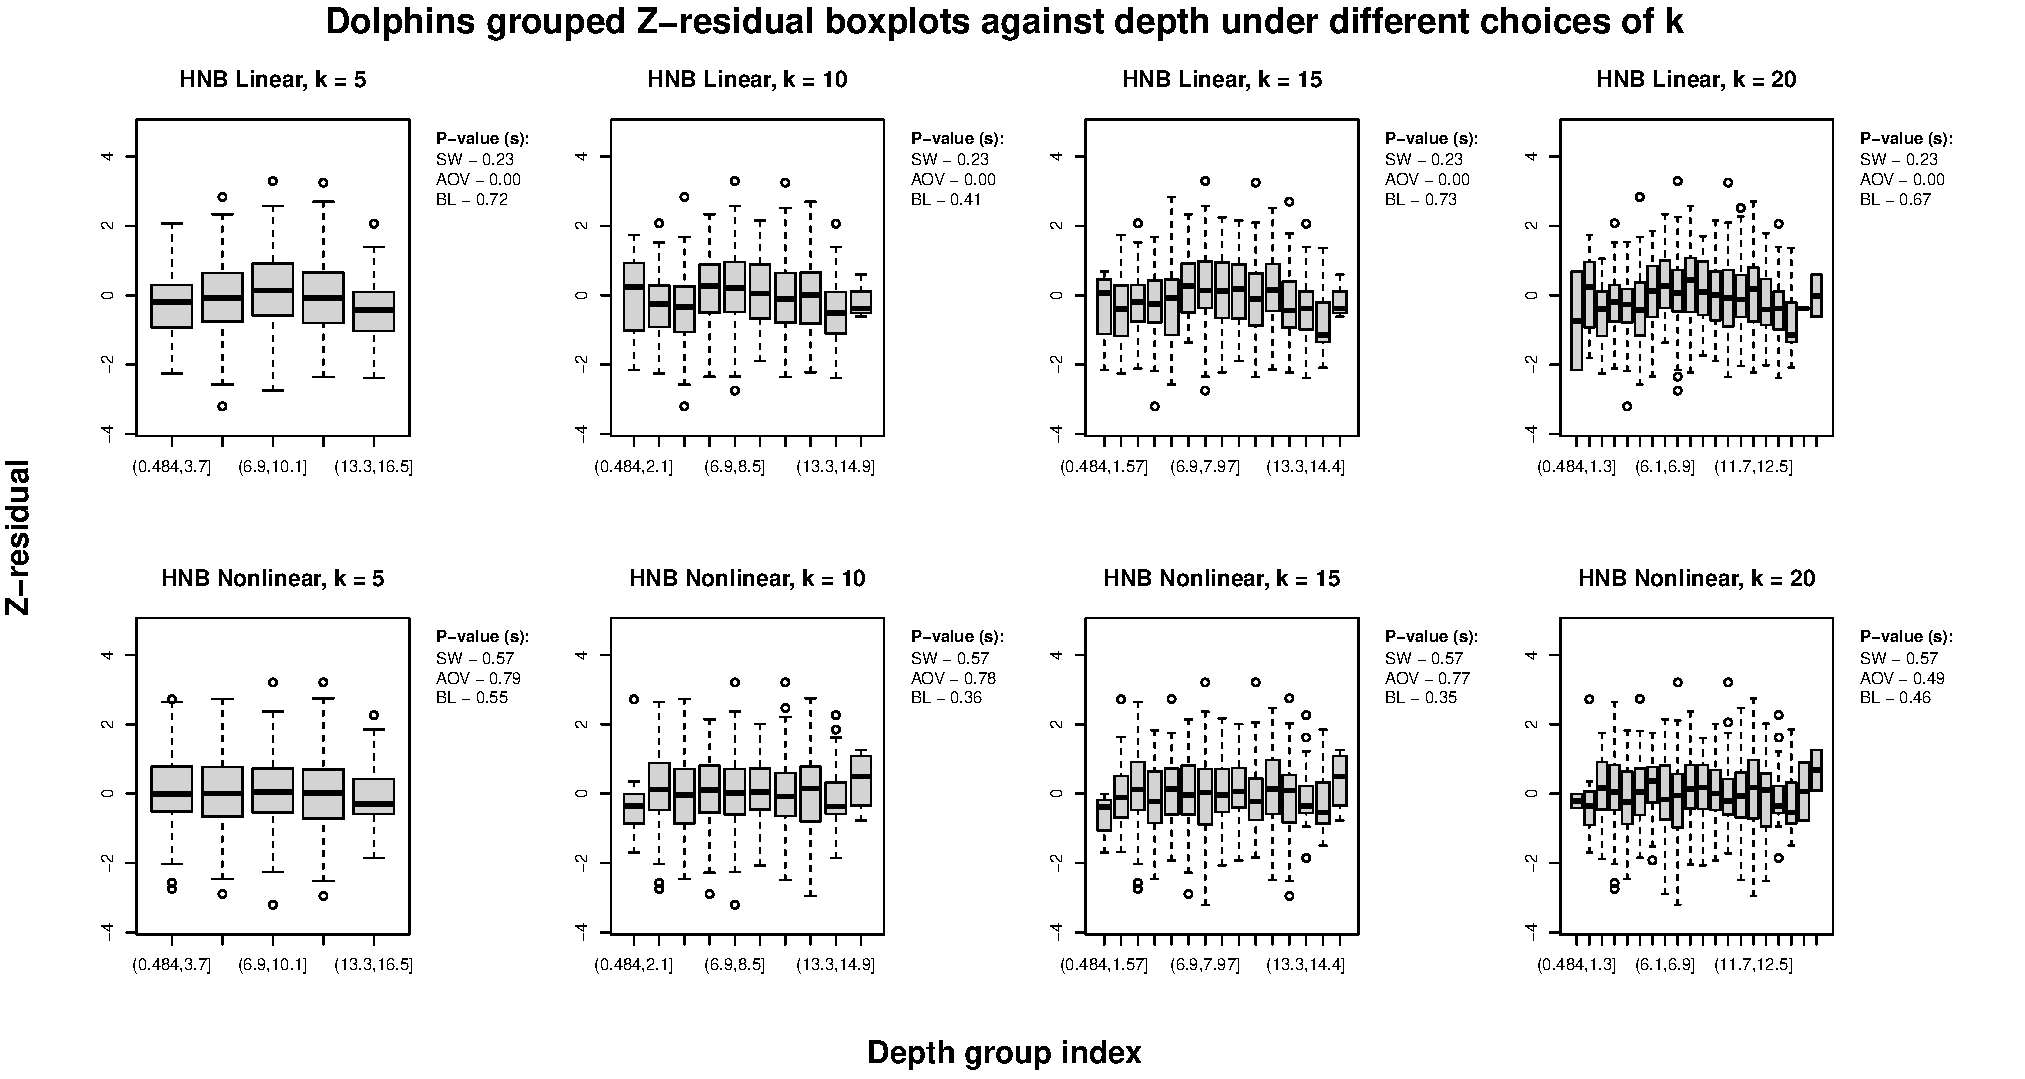
\includegraphics[width=\textwidth, height=\textwidth]{plot/appendix_binning_sensitivity_boxplots_HNB.pdf}
\caption{Grouped posterior RSP Z-residual boxplots against depth for the linear (top) and nonlinear (bottom) HNB models, evaluated under varying numbers of equally spaced intervals ($k$).}
\label{fig_binning_sensitivity}
\end{figure}

Table~\ref{tab:binning_sensitivity_pbound} reports these upper-bound $p$-values. Across all $k$, the linear HNB model consistently exhibits a residual mean pattern against depth, whereas the nonlinear model shows no remaining grouped differences. This confirms our depth diagnostic conclusions are robust to the default choice of $k=10$.

\begin{table}[!htbp]
\centering
\caption{Sensitivity of the Z-AOV test to the number of depth groups ($k$) for the dolphin-sighting data. Smaller $p$-values indicate stronger evidence of residual mean differences. The default choice used in the main text is $k=10$.}
\label{tab:binning_sensitivity_pbound}
\small
\setlength{\tabcolsep}{5pt}
\renewcommand{\arraystretch}{1.15}
\begin{tabular}{lcccc}
\toprule
Model 
& $k=5$  & $k=10$ & $k=15$ & $k=20$ \\
\midrule
Linear HNB 
& 0.006 & 0.015 & 0.047  & 0.039  \\
Nonlinear HNB 
& 1.000 & 1.000 & 1.000 & 1.000  \\
\bottomrule
\end{tabular}
\end{table}


\clearpage

% \subsection{Numerical Illustration of Replicated $p$-values}
% \label{sec:repl_pvalue_illustration}

% To provide a numerical summary of the replicated $p$-value histograms discussed in Section~\ref{M-upper_bound} of the main text, we summarize the replicated AOV $p$-values from the dolphin-sighting analysis. The corresponding replicated $p$-value histograms are shown in Figures~\ref{M-fig-realdata_linear_plot}(c,d) and~\ref{M-fig-realdata_nonlinear_plot}(c,d) of the main text. For each model, \(J = 500\) auxiliary randomizations were used.


% \begin{table}[htbp]
% \centering
% \caption{Numerical summary of replicated AOV $p$-values against depth for the dolphin-sighting data. The expected count under uniform replicated $p$-values is \(500 \times 0.05 = 25\).}
% \label{tab:repl_pvalue_summary}
% \begin{tabular}{lrrrr}
% \toprule
% Model & $J$ & $\#\{p \le 0.05\}$ & Proportion & Median upper-bound $p$-value \\
% \midrule
% Linear HNB & 500 & 405 & 0.81 & 0.014 \\
% Nonlinear HNB & 500 & 5 & 0.01 & 1.000 \\
% \bottomrule
% \end{tabular}
% \end{table}

\clearpage


\section{Asymptotic Properties of Z-residuals}\label{supp:proofs}

\subsection{Illustration of the Uniformity of RSP}\label{rspill}
We illustrate the uniformity of RSP using a toy example. We consider a Hurdle Exponential model, for which the survival function, $S(y)$, and probability mass function (PMF), $p(y)$, are defined as:
\begin{equation}
S(y) = \begin{cases}
1 & \text{if } y < 0 \\
(1 - p_0) \cdot e^{-\lambda y} & \text{if } y \ge 0
\end{cases}
\quad \text{and} \quad
p(y) = \begin{cases}
p_0 & \text{if } y = 0 \\
0 & \text{if } y \neq 0
\end{cases}
\end{equation}
\begin{figure}[htp]
\centering
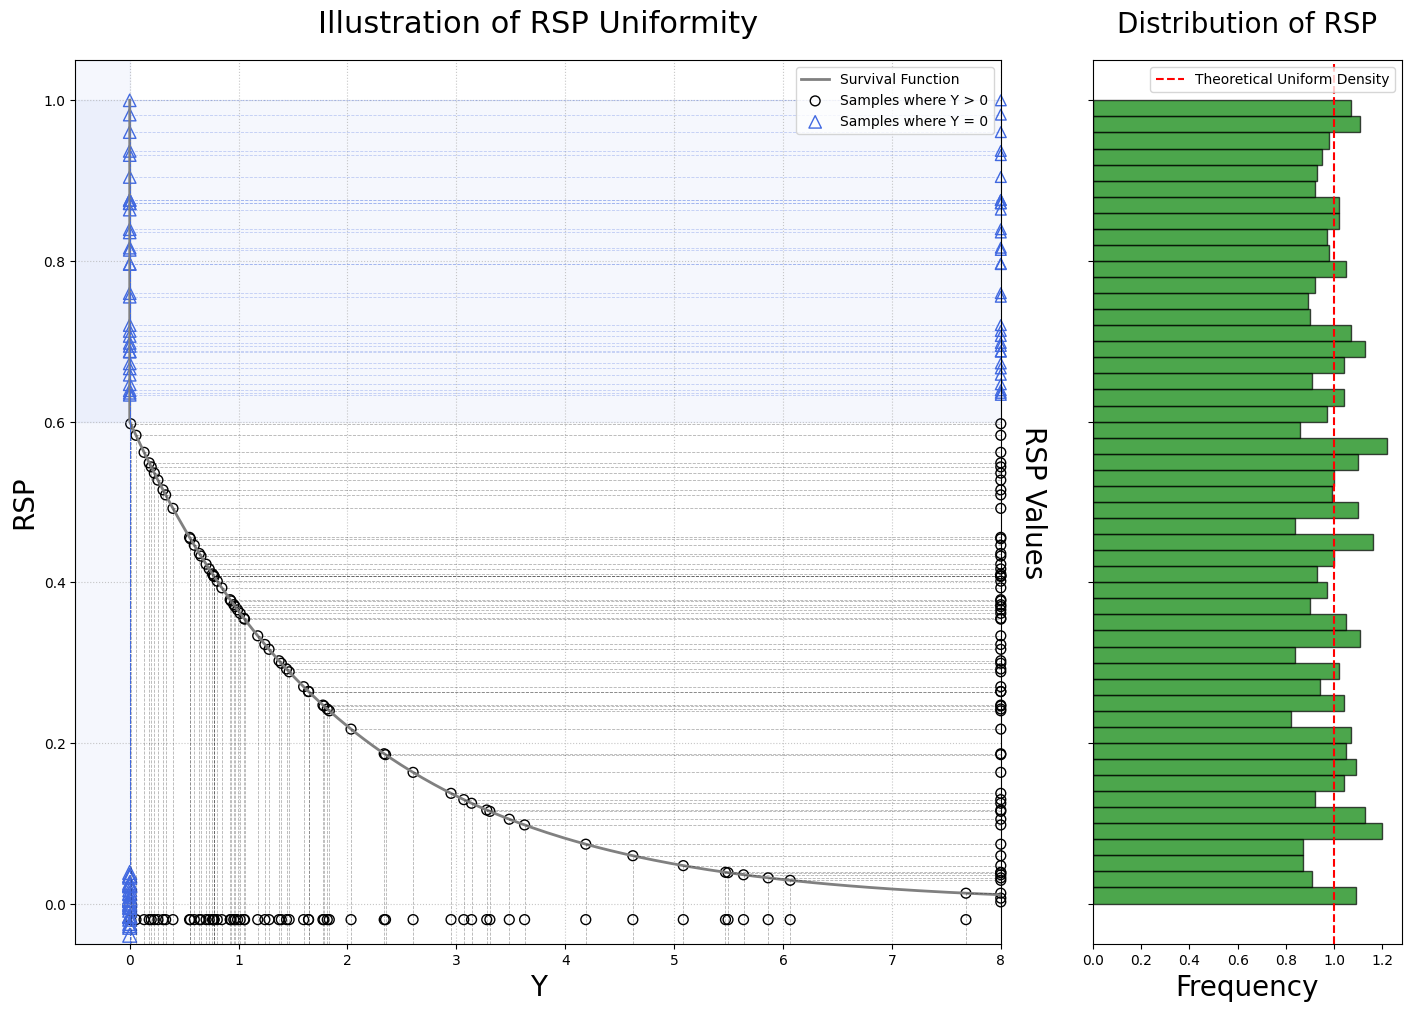
\includegraphics[width=.8\textwidth, height=0.5\textwidth]{plot/rspillstration.png}
\caption{The plot displays the survival function alongside randomized survival probabilities (RSP) for a discrete distribution. The histogram on the right shows the distribution of 5000 RSP values.}
\label{fig:rsp}
\end{figure}

Figure~\ref{fig:rsp} (left panel) shows the survival function for this model, which has a discrete jump at $y=0$ corresponding to the probability mass $p_0$. To illustrate the theorem, we generated 5000 observations ($y_i$) from this distribution and computed the Randomized Survival Probability (RSP) for each. The calculation depends on the value of the observation. For an observation from the continuous part ($y_i>0$), where the probability mass $p(y_i)=0$, the RSP is simply its survival probability, $\text{RSP}_i = S(y_i)$; this deterministic mapping is shown by the hollow circles. For an observation from the discrete part ($y_i=0$), the RSP is calculated as $\text{RSP}_i = S(0) + U_i \cdot p_0$, using a random draw $U_i \sim \text{Unif}(0,1)$. As shown by the triangles, this process randomly maps each observation where $y_i=0$ to a uniform value within the interval $[S(0), 1]$, effectively distributing the probability mass $p_0$ across this range (the shaded blue region). The right panel of Figure~\ref{fig:rsp} displays the histogram of all 5000 calculated RSP values, which closely follows a uniform distribution on $(0,1)$.

 

\subsection{Proof of the Uniformity of RSP Under the True Model}
\begin{theorem}[Uniformity of the Randomized Survival Probability]
Let $Y$ be any random variable on $\mathbb{R}$ with survival function $S(y) = P(Y>y)$ and probability mass function $p(y) = P(Y=y)$, which is 0 when $S(y)$ is continuous at $y$. Let $U \sim \text{Uniform}(0,1)$ be independent of $Y$. Then the Randomized Survival Probability (RSP), defined as
\begin{equation}
V = S(Y) + U \cdot p(Y),
\end{equation}
is a standard uniform random variable, i.e., $V \sim \text{Uniform}(0,1)$.
\label{thm:rspunif}
\end{theorem}

\begin{proof}
To prove that $V$ is a standard uniform random variable, we will show that for any interval $A \subseteq [0,1]$, the probability $P(V \in A)$ is equal to its length (Lebesgue measure), $\lambda(A)$. The proof proceeds in four steps.
\begin{proofpart}[Setup and Conditional Expectation]
We express the probability $P(V \in A)$ using the law of total expectation:
\begin{equation}
P(V \in A) = \E[\mathbf{1}_{A}(V)] = \E \left[ \E[\mathbf{1}_{A}(S(Y) + U \cdot p(Y)) \mid Y] \right]
\end{equation}
Let's analyze the inner conditional expectation, which we denote $g(y) = E_U[\mathbf{1}_{A}(S(y) + U \cdot p(y))]$. For any fixed $y$, the conditional random variable $V \mid Y=y$ is uniformly distributed on the interval $I_y^V = [S(y), S(y)+p(y)]$. Let $D = \{y_k : p(y_k) > 0\}$ be the set of discrete mass points of $Y$.
\begin{itemize}
    \item \textbf{For a discrete point $y_k \in D$}, the interval $I_{y_k}^V$ has length $p(y_k) > 0$. The conditional expectation is the probability that a uniform variable on this interval falls in $A$:
    \begin{equation}
    g(y_k) = \frac{\lambda(A \cap I_{y_k}^V)}{\lambda(I_{y_k}^V)} = \frac{\lambda(A \cap I_{y_k}^V)}{p(y_k)}
\end{equation}
    \item \textbf{For a continuous point $y \notin D$}, we have $p(y)=0$. The interval $I_y^V$ collapses to a single point, and the conditional expectation becomes:
    \begin{equation}
    g(y) = \E[\mathbf{1}_{A}(S(y))] = \mathbf{1}_{A}(S(y))
\end{equation}
\end{itemize}
\end{proofpart}

\begin{proofpart}[Contribution from Discrete Points]
We now evaluate the outer expectation by first integrating over the discrete part of $Y$'s distribution. This contribution is a sum:
\begin{equation}
\int_{D} g(y) \, dF(y) = \sum_{y_k \in D} g(y_k) p(y_k) = \sum_{y_k \in D} \left( \frac{\lambda(A \cap I_{y_k}^V)}{p(y_k)} \right) p(y_k) = \sum_{y_k \in D} \lambda(A \cap I_{y_k}^V)
\end{equation}
\end{proofpart}

\begin{proofpart}[Contribution from Continuous Points]
Next, we integrate over the continuous part of the distribution, $C = \mathbb{R} \setminus D$. Let the density function on this set be $f_c(y)$.
\begin{equation}
\int_{C} g(y) \, dF(y) = \int_{C} \mathbf{1}_{A}(S(y)) f_c(y) \, dy
\end{equation}
We perform a change of variables from $y$ to $v = S(y)$, for which the differential is $dv = -S'(y)dy = -(-f_c(y))dy = f_c(y)dy$. As $y$ sweeps across the set $C$, the variable $v=S(y)$ sweeps across the set $I_C^V = [0,1] \setminus \bigcup_{k} I_{y_k}^V$. The integral becomes:
\begin{equation}
\int_{I_C^V} \mathbf{1}_{A}(v) \, dv = \lambda(A \cap I_C^V)
\end{equation}
\end{proofpart}

\begin{proofpart}[Conclusion]
Finally, we add the contributions from the discrete and continuous parts:
\begin{equation}
P(V \in A) = \sum_{y_k \in D} \lambda(A \cap I_{y_k}^V) + \lambda(A \cap I_C^V)
\end{equation}
The sets $\{I_{y_k}^V\}_{y_k \in D}$ and $I_C^V$ form a partition of the unit interval $[0,1]$. Therefore, their intersections with the set $A$ form a partition of $A$. The sum of the lengths of these disjoint intersecting sets is simply the total length of $A$:
\begin{equation}
P(V \in A) = \lambda\left(\left(\bigcup_{k} (A \cap I_{y_k}^V)\right) \cup (A \cap I_C^V)\right) = \lambda(A)
\end{equation}
Since $P(V \in A) = \lambda(A)$ for any Borel set $A \subseteq [0,1]$, the random variable $V$ is, by definition, uniformly distributed on $[0,1]$.
\end{proofpart}
\end{proof}


\subsection{Asymptotic Uniformity of the CV and Posterior RSP}

\begin{theorem}[Total Variation Convergence of the LOO Predictive Distribution]
\label{thm:loo-pred-tv-formal-w0}
Let $Y_1,\dots,Y_{n+1}$ be independent random variables with true probability laws $P_i^{(*)}$ possessing densities $f_i^{(*)}$. Consider a statistical model $\{f_i(\cdot\mid\theta):\theta\in\Theta\}$ and a prior law $\Pi$. Assume the model is well-specified, meaning the set of true parameters
\begin{equation}W_0 = \{\theta \in \Theta : f_i(\cdot \mid \theta) = f_i^{(*)} \text{ for all } i\}\end{equation}
is non-empty. Let $\theta^\star$ be any representative element from $W_0$.

For each $i$, let $\Pi(\cdot\mid\mathbf Y_{-i})$ be the posterior law based on the LOO sample $\mathbf Y_{-i}$ of size $n$. The LOO predictive density is $f_i^{(n),\mathrm{CV}}(y)\;=\;\int_{\Theta} f_i(y\mid\theta)\,d\Pi(\theta\mid\mathbf Y_{-i})$. Let $\bar K_{n,-i}(\theta,\theta^\star)$ and $\bar h_{n,-i}(\theta,\theta^\star)$ be the average KL divergence and Hellinger distance from the true distribution. Assume the following conditions hold for some sequence $\varepsilon_n\downarrow 0$ and sieves $\Theta_n \subset \Theta$:
\begin{enumerate}
    \item[\textnormal{(i)}] Measurability: The function $(y, \theta) \mapsto f_i(y \mid \theta)$ is measurable for each $i$.

    \item[\textnormal{(ii)}] Prior Mass Condition: The prior law assigns sufficient mass to Kullback-Leibler neighborhoods of the true parameter set $W_0$, i.e., for some constant $C>0$:
    \begin{equation}\Pi(\{\theta:\bar K_{n,-i}(\theta,\theta^\star)\le \varepsilon_n^2\}) \ge e^{-C n\varepsilon_n^2}.\end{equation}

    \item[\textnormal{(iii)}] Existence of Tests: There exist uniformly consistent tests for Hellinger neighborhoods of $W_0$. That is, for every $\delta>0$, there exists a sequence of tests $\phi_n$ and a constant $c>0$ such that for large $n$:
    \begin{equation} \mathbb{E}_{\theta^\star}\phi_n \le e^{-cn\varepsilon_n^2} \quad \text{and} \quad \sup_{\{\theta \in \Theta_n : \bar{h}_{n,-i}(\theta,\theta^\star) > \delta\}} \mathbb{E}_{\theta}(1-\phi_n) \le e^{-cn\varepsilon_n^2}.\end{equation}

    \item[\textnormal{(iv)}] Complexity Control: The parameter space has controlled complexity, meaning the entropy of the sieves does not grow too quickly and the prior mass outside the sieves is exponentially small:
    \begin{equation} \log N(\varepsilon_n, \Theta_n, \bar h_{n,-i})\le C n\varepsilon_n^2 \quad \text{and} \quad \Pi(\Theta_n^c) \le e^{-D n\varepsilon_n^2},\end{equation}
    for constants $C,D > 0$, where the term $N(\varepsilon_n, \Theta_n, \bar h_{n,-i})$ denotes the covering number indicating the complexity of a model, see \citet{ghosal2007convergence} for precise definition.

    \item[\textnormal{(v)}] $L^1$ Continuity: For each fixed $i$, the map $\theta \mapsto f_i(\cdot\mid\theta)$ is continuous in the $L^1(\mu)$ norm on a neighborhood of the set $W_0$. That is, for every $\epsilon>0$, there exists an open set $U_\epsilon$ containing $W_0$ such that $\sup_{\theta\in U_\epsilon}\,\|f_i(\cdot\mid\theta)-f_i^{(*)}\|_{L^1(\mu)}<\epsilon$.
\end{enumerate}
Then for each fixed $i$, as $n\to\infty$, the LOO predictive distribution converges to the true distribution in total variation, in probability:
\begin{equation}\big\|P_i^{(n),\mathrm{CV}}-P_i^{(*)}\big\|_{\mathrm{TV}} \xrightarrow{P} 0.\end{equation}
\end{theorem}

\begin{proof}
The cornerstone of the proof is posterior consistency with respect to the true parameter set $W_0$. Conditions (i)–(iv) are sufficient for Schwartz-type theorems \citep{ghosal2007convergence, Choi2008Remarks}, which guarantee that the LOO posterior law $\Pi(\cdot \mid \mathbf{Y}_{-i})$ concentrates on Hellinger neighborhoods of the true density. In the parameter space, this means the posterior concentrates on the set of parameters that produce the true density, which is exactly $W_0$. Formally, for any open set $U$ containing the set $W_0$, it follows that:
\begin{equation} \label{eq:post-consistency-w0}
\Pi(U^c\mid\mathbf Y_{-i}) \xrightarrow{P} 0 \quad \text{as } n\to\infty.
\end{equation}

With this rigorous consistency result, we now prove the convergence of the predictive distribution. Let $\Delta_n := \|f_i^{(n),\mathrm{CV}}-f_i^{(*)}\|_{L^1(\mu)}$. Our goal is to show $\Delta_n \xrightarrow{P} 0$.

By the triangle inequality, we bound $\Delta_n$ by the posterior expectation of the $L^1$ error:
\begin{equation}\Delta_n \le \int_{\Theta} \|f_i(\cdot\mid\theta)-f_i^{(*)}\|_{L^1(\mu)}\,d\Pi(\theta\mid\mathbf Y_{-i}).\end{equation}For any $\epsilon > 0$, Condition (v) guarantees the existence of an open neighborhood $U_\epsilon$ containing the entire set $W_0$ where $\|f_i(\cdot\mid\theta)-f_i^{(*)}\|_{L^1(\mu)} < \epsilon$. Decomposing the integral over this $U_\epsilon$ and its complement yields:\begin{equation}\Delta_n \le \int_{U_\epsilon} \epsilon \,d\Pi(\theta\mid\mathbf Y_{-i}) + \int_{U_\epsilon^c} 2 \,d\Pi(\theta\mid\mathbf Y_{-i}) \le \epsilon + 2\,\Pi(U_\epsilon^c\mid\mathbf Y_{-i}).\end{equation}
Since $U_\epsilon$ is an open set containing $W_0$, our consistency result from \eqref{eq:post-consistency-w0} directly implies that $\Pi(U_\epsilon^c\mid\mathbf Y_{-i}) = o_P(1)$. Thus, for any arbitrarily small $\epsilon > 0$,\begin{equation}\Delta_n \le \epsilon + o_P(1).\end{equation}

This implies that $\Delta_n \xrightarrow{P} 0$, which completes the proof.
\end{proof}


\begin{theorem}[Asymptotic Uniformity of the Cross-Validated RSP]
\label{thm:cvrsp-unif}
Under the same setup and conditions specified in Theorem \ref{thm:loo-pred-tv-formal-w0}, let $S_i^{(n),\mathrm{CV}}(\cdot \mid \mathbf{Y}_{-i})$ and $p_i^{(n),\mathrm{CV}}(\cdot \mid \mathbf{Y}_{-i})$ be the survival function and probability mass function, respectively, corresponding to the LOO predictive density $f_i^{(n),\mathrm{CV}}$.

The cross-validated Randomized Survival Probability ($\mathrm{RSP}$) for observation $Y_i$ is defined as:
\begin{equation}
\mathrm{RSP}_i^{(n),\mathrm{CV}} = S_i^{(n),\mathrm{CV}}(Y_i \mid \mathbf{Y}_{-i}) + U_i \cdot p_i^{(n),\mathrm{CV}}(Y_i \mid \mathbf{Y}_{-i}), \quad \text{where } U_i \stackrel{\text{i.i.d.}}{\sim} \mathrm{Unif}(0,1)
\end{equation}

Then, as $n\to\infty$, the cross-validated RSP converges in distribution to a standard uniform random variable:\begin{equation} \mathrm{RSP}_i^{(n),\mathrm{CV}} \Rightarrow \mathrm{Unif}(0,1).\end{equation}

\end{theorem}

\begin{proof}
The proof is established in four parts. We first state the key result from Theorem \ref{thm:loo-pred-tv-formal-w0}, then show that the $\mathrm{RSP}_i^{(n),\mathrm{CV}}$ converges in probability to a known uniform random variable, and finally conclude with Slutsky's theorem.

\begin{proofpart}[Convergence in Total Variation]
The conditions assumed in Theorem \ref{thm:loo-pred-tv-formal-w0} are sufficient to guarantee that the LOO predictive distribution, $P_i^{(n),\mathrm{CV}}$, converges to the true data-generating distribution, $P_{i}^{(*)}$, in total variation (TV) distance, in probability. That is,
\begin{equation}
\|P_i^{(n),\mathrm{CV}} - P_{i}^{(*)}\|_{\mathrm{TV}}\ \xrightarrow{P}\ 0 \quad \text{as} \quad n\to\infty.
\label{eq:tv_convergence_recap}
\end{equation}
\end{proofpart}

\begin{proofpart}[Bounding the Difference Between the RSP and Its Limit]
Our goal is to show that $\mathrm{RSP}_i^{(n),\mathrm{CV}}$ converges in distribution to a Unif0,1) random variable. We begin by defining this target variable as $V_i := S_{i}^{(*)}(Y_i) + U_i p_{i}^{(*)}(Y_i)$, where $S_{i}^{(*)}$ and $p_{i}^{(*)}$ are the survival function and PMF of the true distribution $P_{i}^{(*)}$. By the probability integral transform, $V_i$ is exactly distributed as $\mathrm{Unif}(0,1)$.

We now bound the absolute difference between the RSP and its target, $D_n := |\mathrm{RSP}_i^{(n),\mathrm{CV}} - V_i|$, using the triangle inequality:
\begin{equation}
D_n \le \big| S_i^{(n),\mathrm{CV}}(Y_i \mid \mathbf{Y}_{-i}) - S_{i}^{(*)}(Y_i) \big| + \big| p_i^{(n),\mathrm{CV}}(Y_i \mid \mathbf{Y}_{-i}) - p_{i}^{(*)}(Y_i) \big|.
\label{eq:difference_bound_detailed}
\end{equation}
\end{proofpart}

\begin{proofpart}[Convergence of the Bounded Components]
We now show that the bound in \eqref{eq:difference_bound_detailed} converges to zero in probability by leveraging the TV convergence from \eqref{eq:tv_convergence_recap}.

\begin{itemize}
    \item \textbf{Survival Term:} The maximum absolute difference between two survival functions is bounded by the total variation distance between their corresponding probability measures. Thus, for any value $y$,
    \begin{equation}|S_i^{(n),\mathrm{CV}}(y \mid \mathbf{Y}_{-i}) - S_{i}^{(*)}(y)| \le \|P_i^{(n),\mathrm{CV}} - P_{i}^{(*)}\|_{\mathrm{TV}}.\end{equation}

    Since the TV distance converges to zero in probability, the first term in the bound, evaluated at the random observation $Y_i$, also converges to zero in probability.

    \item \textbf{PMF Term:} Similarly, the absolute difference between two probability mass functions at any single point is also bounded by the TV distance. For continuous distributions, both $p_i^{(n),\mathrm{CV}}$ and $p_{i}^{(*)}$ are zero. In either case, the second term in the bound converges to zero in probability.
\end{itemize}
Since both terms on the right-hand side of \eqref{eq:difference_bound_detailed} converge to zero in probability, their sum, which is the upper bound for $D_n$, must also converge to zero in probability.
\end{proofpart}

\begin{proofpart}[Conclusion via Slutsky's Theorem]
From the previous step, we have established that $|\mathrm{RSP}_i^{(n),\mathrm{CV}} - V_i| \xrightarrow{P} 0$, which is equivalent to the statement that the sequence of random variables $\mathrm{RSP}_i^{(n),\mathrm{CV}} - V_i$ converges to 0 in probability. By Slutsky's theorem, $\mathrm{RSP}_i^{(n),\mathrm{CV}}$ must converge in distribution to the same limit as $V_i$. Therefore, we conclude that:
\begin{equation}\mathrm{RSP}_i^{(n),\mathrm{CV}} \ \Rightarrow\ \mathrm{Unif}(0,1).\end{equation}

\end{proofpart}
\end{proof}
\begin{theorem}[Asymptotic Uniformity of the Posterior RSP]
\label{thm:postrspunif}
Under the same setup and conditions specified in Theorem \ref{thm:loo-pred-tv-formal-w0}, let the full sample be $\mathbf{Y} = (Y_1, \dots, Y_{n+1})$. For any fixed $i \in \{1, \dots, n+1\}$, let the full-data posterior predictive distribution for $Y_i$ be denoted $P_i^{(n+1),\mathrm{post}}$, with density $f_i^{(n+1),\mathrm{post}}(y_i \mid \mathbf{Y})$. Let $S_i^{(n+1),\mathrm{post}}$ and $p_i^{(n+1),\mathrm{post}}$ be the corresponding survival function and PMF.

The posterior Randomized Survival Probability ($\mathrm{RSP}$) is defined as:
\begin{equation}\mathrm{RSP}_i^{(n+1),\mathrm{post}} \;=\; S_i^{(n+1),\mathrm{post}}(Y_i \mid \mathbf{Y})\;+\;U_i \cdot p_i^{(n+1),\mathrm{post}}(Y_i \mid \mathbf{Y})\end{equation}

where $U_i \sim \mathrm{Unif}(0,1)$ is an independent random variable.

Then, for each fixed $i$, as $n\to\infty$, the posterior RSP converges in distribution to a standard uniform random variable:
\begin{equation}\mathrm{RSP}_i^{(n+1),\mathrm{post}} \ \Rightarrow\ \mathrm{Unif}(0,1).\end{equation}

\end{theorem}

\begin{proof}
The proof demonstrates that the posterior RSP is asymptotically equivalent to the cross-validated RSP from Theorem \ref{thm:cvrsp-unif}, whose asymptotic uniformity has already been established.

\begin{proofpart}[Convergence of Predictive Distributions]
The conditions of Theorem \ref{thm:loo-pred-tv-formal-w0} ensure that any posterior predictive distribution based on a sufficiently large sample will converge to the true data-generating distribution. This applies to both the full-data posterior predictive (based on $n+1$ points) and the leave-one-out (LOO) predictive (based on $n$ points). As $n \to \infty$, both converge to the true distribution $P_i^{(*)}$ in total variation:
\begin{equation}\|P_i^{(n+1),\mathrm{post}} - P_i^{(*)}\|_{\mathrm{TV}} \xrightarrow{P} 0 \quad \text{and} \quad \|P_i^{(n),\mathrm{CV}} - P_i^{(*)}\|_{\mathrm{TV}} \xrightarrow{P} 0.\end{equation}

By the triangle inequality, the distance between the full-data and LOO predictive distributions must therefore also converge to zero:
\begin{equation}
\|P_i^{(n+1),\mathrm{post}} - P_i^{(n),\mathrm{CV}}\|_{\mathrm{TV}} \le \|P_i^{(n+1),\mathrm{post}} - P_i^{(*)}\|_{\mathrm{TV}} + \|P_i^{(*)} - P_i^{(n),\mathrm{CV}}\|_{\mathrm{TV}} \xrightarrow{P} 0.
\label{eq:tv_equiv}
\end{equation}
\end{proofpart}

\begin{proofpart}[Asymptotic Equivalence of RSPs]
Next, we show that the difference between the posterior RSP and the cross-validated RSP vanishes asymptotically. This difference, $D_n := \mathrm{RSP}_i^{(n+1),\mathrm{post}} - \mathrm{RSP}_i^{(n),\mathrm{CV}}$, can be bounded by the TV distance between the two predictive distributions:
\begin{align*}
|D_n| &= \left| \left(S_i^{(n+1),\mathrm{post}}(Y_i|\mathbf{Y}) - S_i^{(n),\mathrm{CV}}(Y_i|\mathbf{Y}_{-i})\right) + U_i \left(p_i^{(n+1),\mathrm{post}}(Y_i|\mathbf{Y}) - p_i^{(n),\mathrm{CV}}(Y_i|\mathbf{Y}_{-i})\right) \right| \\
&\le \left| S_i^{(n+1),\mathrm{post}}(Y_i|\mathbf{Y}) - S_i^{(n),\mathrm{CV}}(Y_i|\mathbf{Y}_{-i}) \right| + \left| p_i^{(n+1),\mathrm{post}}(Y_i|\mathbf{Y}) - p_i^{(n),\mathrm{CV}}(Y_i|\mathbf{Y}_{-i}) \right| \\
&\le 2 \cdot \|P_i^{(n+1),\mathrm{post}} - P_i^{(n),\mathrm{CV}}\|_{\mathrm{TV}}.
\end{align*}
From the result in \eqref{eq:tv_equiv}, the TV distance on the right converges to zero in probability. Therefore, $|D_n| \xrightarrow{P} 0$, which gives us the key asymptotic equivalence:
\begin{equation}
\mathrm{RSP}_i^{(n+1),\mathrm{post}} - \mathrm{RSP}_i^{(n),\mathrm{CV}} \xrightarrow{P} 0.
\label{eq:rsp_equiv}
\end{equation}
\end{proofpart}

\begin{proofpart}[Conclusion via Slutsky's Theorem]
We can express the posterior RSP as the sum of two terms: the cross-validated RSP and a residual term that converges to zero in probability. From \eqref{eq:rsp_equiv}, we have:
\begin{equation}\mathrm{RSP}_i^{(n+1),\mathrm{post}} = \mathrm{RSP}_i^{(n),\mathrm{CV}} + o_P(1).\end{equation}
We have already proven in Theorem \ref{thm:cvrsp-unif} that the cross-validated RSP converges in distribution to a standard uniform variable:\begin{equation} \mathrm{RSP}_i^{(n),\mathrm{CV}} \Rightarrow \mathrm{Unif}(0,1).\end{equation}

By Slutsky's Theorem, the sum of a sequence of random variables that converges in distribution and another that converges in probability to zero will converge in distribution to the same limit. Therefore, we conclude that:
\begin{equation}
\mathrm{RSP}_i^{(n+1),\mathrm{post}} \ \Rightarrow\ \mathrm{Unif}(0,1).
\label{eq:final_conv_post}
\end{equation}
\end{proofpart}
\end{proof}

\subsection{Asymptotic Independence of the Posterior and CV RSPs}

\begin{theorem}[Asymptotic Independence of Cross-Validated RSPs]\label{sec:rspindep}

\label{thm:cvrspindep}

Under the same assumptions as the previous theorem (for independent, non-i.i.d. data), for any fixed pair of distinct indices $i \neq j$, the random vector of cross-validated Randomized Survival Probabilities converges in distribution to a pair of independent standard uniform random variables. Formally, as the sample size $n\to\infty$:
\begin{equation}
    (\text{RSP}_i^{(n),\text{CV}}, \text{RSP}_j^{(n),\text{CV}}) \ \Rightarrow\ (\text{Uniform}(0,1), \text{Uniform}(0,1))
\end{equation}
where the two uniform random variables in the limiting distribution are independent.
\end{theorem}

\begin{proof}
The proof strategy is to show that the random vector $(\text{RSP}_i^{(n),\text{CV}}, \text{RSP}_j^{(n),\text{CV}})$ converges in distribution to the vector of RSPs under the true parameters, $(V_i, V_j)$. Since $Y_i$ and $Y_j$ are independent, the limiting variables $V_i$ and $V_j$ will be independent, establishing the theorem.

\begin{proofpart}[Component-wise Convergence in Probability]
In the proof of the previous theorem, we established that for any fixed $i$, the absolute difference between the estimated RSP and its true-parameter counterpart converges to zero in probability. Let $V_i := S_{i}^{(*)}(Y_i)+U_i p_{i}^{(*)}(Y_i)$ and $V_j := S_{j}^{(*)}(Y_j)+U_j p_{j}^{(*)}(Y_j)$. We have already shown:
\begin{equation}
|\text{RSP}_i^{(n),\text{CV}} - V_i| \xrightarrow{P} 0
\end{equation}
and by identical logic for index $j$:
\begin{equation}
|\text{RSP}_j^{(n),\text{CV}} - V_j| \xrightarrow{P} 0.
\end{equation}
\end{proofpart}

\begin{proofpart}[Joint Convergence in Probability]
Consider the 2-dimensional random vector formed by the differences:
\begin{equation}
\mathbf{D}_n = \left( \text{RSP}_i^{(n),\text{CV}} - V_i, \quad \text{RSP}_j^{(n),\text{CV}} - V_j \right).
\end{equation}
A random vector converges in probability to a constant vector if and only if each of its components converges in probability to the corresponding component of the constant vector \citep[Thm 1.9]{shao2008}. Since we established in Step 1 that each component of $\mathbf{D}_n$ converges in probability to 0, the vector itself converges in probability to the zero vector:
\begin{equation}
\mathbf{D}_n \xrightarrow{P} (0,0).
\label{eq:joint_conv_p}
\end{equation}
\end{proofpart}

\begin{proofpart}[Independence of the Limiting Variables]
The limiting random vector is $(V_i, V_j)$. By definition, $V_i$ is a function of only $(Y_i, U_i)$ and $V_j$ is a function of only $(Y_j, U_j)$. By the theorem's initial setup, for $i \neq j$, the random variables $Y_i$ and $Y_j$ are independent. The auxiliary variables $U_i$ and $U_j$ are also independent of each other and of all $Y$ variables. Since $V_i$ and $V_j$ are functions of disjoint sets of independent random variables, they are themselves independent. Each is marginally distributed as $\text{Uniform}(0,1)$.
\end{proofpart}

\begin{proofpart}[Conclusion via Multivariate Slutsky's Theorem]
We can write the vector of estimated RSPs as the sum of the true RSP vector and the difference vector $\mathbf{D}_n$:
\begin{equation}
(\text{RSP}_i^{(n),\text{CV}}, \text{RSP}_j^{(n),\text{CV}}) = (V_i, V_j) + \mathbf{D}_n.
\end{equation}
We have established that the distribution of $(V_i, V_j)$ is a pair of independent $\text{Uniform}(0,1)$ variables, and that $\mathbf{D}_n \xrightarrow{P} (0,0)$. By the multivariate version of Slutsky's theorem, the vector $(\text{RSP}_i^{(n),\text{CV}}, \text{RSP}_j^{(n),\text{CV}})$ must converge in distribution to the same limit as $(V_i, V_j)$.

\end{proofpart}
\end{proof}
\begin{theorem}[Asymptotic Independence of Posterior RSPs]
\label{thm:postrspindep}
Under the same setup and conditions as in Theorem \ref{thm:loo-pred-tv-formal-w0}, for any fixed pair of distinct indices $i \neq j$, the random vector of posterior RSPs converges in distribution to a pair of independent standard uniform random variables.

Formally, as $n\to\infty$:
\begin{equation}(\mathrm{RSP}_i^{(n+1),\mathrm{post}}, \mathrm{RSP}_j^{(n+1),\mathrm{post}}) \ \Rightarrow\ (\mathrm{Unif}(0,1), \mathrm{Unif}(0,1))\end{equation}
where the two uniform random variables in the limiting distribution are independent.
\end{theorem}

\begin{proof}
The proof relies on the multivariate Slutsky's theorem. We first establish that the vector of posterior RSPs is asymptotically equivalent to the vector of cross-validated RSPs.

From the proof of Theorem \ref{thm:postrspunif}, we know that for any single observation $k$, the difference between the posterior and cross-validated RSP converges to zero in probability: $\mathrm{RSP}_k^{(n+1),\mathrm{post}} - \mathrm{RSP}_k^{(n),\mathrm{CV}} \xrightarrow{P} 0$. Since convergence in probability for a random vector is equivalent to component-wise convergence \citep{shao2008}, the difference vector also converges in probability to the zero vector:
\begin{equation}\left( \mathrm{RSP}_i^{(n+1),\mathrm{post}} - \mathrm{RSP}_i^{(n),\mathrm{CV}}, \quad \mathrm{RSP}_j^{(n+1),\mathrm{post}} - \mathrm{RSP}_j^{(n),\mathrm{CV}} \right) \xrightarrow{P} (0,0).\end{equation}
This establishes the asymptotic equivalence of the two RSP vectors. Next, we consider the limiting distribution of the cross-validated vector, $(\mathrm{RSP}_i^{(n),\mathrm{CV}}, \mathrm{RSP}_j^{(n),\mathrm{CV}})$. As shown in Theorem \ref{thm:cvrsp-unif}, each component converges in distribution to a standard uniform. Furthermore, $\mathrm{RSP}_i^{(n),\mathrm{CV}}$ is asymptotically a function of only $Y_i$, and $\mathrm{RSP}_j^{(n),\mathrm{CV}}$ is asymptotically a function of only $Y_j$. Because the original observations $Y_i$ and $Y_j$ are independent for $i \neq j$, the RSPs are asymptotically independent. Thus, the vector converges in distribution:
\begin{equation}(\mathrm{RSP}_i^{(n),\mathrm{CV}}, \mathrm{RSP}_j^{(n),\mathrm{CV}}) \ \Rightarrow\ (\mathrm{Unif}(0,1), \mathrm{Unif}(0,1)),
\end{equation}
where the two uniform random variables in the limiting distribution are independent.

We can now write the posterior RSP vector as the sum of a vector that converges in distribution and a vector that converges in probability to zero. By the multivariate Slutsky's theorem, the posterior RSP vector must converge in distribution to the same limit, which concludes the proof.
\end{proof}

\subsection{Asymptotic Uniformity of Tests Based on Z-residuals}

\begin{theorem}[Asymptotic Uniformity of Tests Based on Z-Residuals]
\label{thm:pvalunif}
Let the assumptions of the preceding theorems hold, ensuring that a set of $n$ Randomized Survival Probabilities, $\{\mathrm{RSP}_1, \dots, \mathrm{RSP}_n\}$, are asymptotically independent and identically distributed (i.i.d.) as $\mathrm{Unif}(0,1)$. Define the Z-residuals as $Z_i = \Phi^{-1}(\mathrm{RSP}_i)$, where $\Phi^{-1}$ is the standard normal quantile function.

Let $T^{(n)} = T(Z_1, \dots, Z_n)$ be any test statistic that is a continuous function of the Z-residuals, and assume its distribution under the null hypothesis (where $Z_i^* \sim_{\text{i.i.d.}} N(0,1)$) is continuous. Let $\mathcal{P}^{(n)}$ be the $p$-value from this test.

Then, as $n\to\infty$, the $p$-value converges in distribution to a standard uniform random variable:
\begin{equation}
\mathcal{P}^{(n)} \ \Rightarrow\ \mathrm{Unif}(0,1).
\end{equation}
\end{theorem}

\begin{proof}
The proof follows a chain of transformations, where each step preserves the convergence in distribution.

By assumption, the vector of RSPs converges in distribution to a vector of i.i.d. standard uniform variables. Since the normal quantile function $\Phi^{-1}$ is continuous, the Contunuous Mapping Theorem (CMT) implies that the vector of Z-residuals $(Z_1, \dots, Z_n)$ converges in distribution to a vector of i.i.d. standard normal variables, $(Z_1^*, \dots, Z_n^*)$.

Next, since the test statistic $T(\cdot)$ is also a continuous function, a second application of the CMT shows that the test statistic $T^{(n)} = T(Z_1, \dots, Z_n)$ converges in distribution to its null distribution, $T^{*(n)} = T(Z_1^*, \dots, Z_n^*)$.

Finally, the $p$-value is the survival function of the null distribution evaluated at the test statistic, $\mathcal{P}^{(n)} = S_{T^{*(n)}}(T^{(n)})$. A fundamental result of probability theory states that if $X_n \Rightarrow X_0$ and the distribution of $X_0$ is continuous, then $S_{X_0}(X_n) \Rightarrow \mathrm{Unif}(0,1)$. Applying this to our case, where $T^{(n)} \Rightarrow T^{*(n)}$ and the distribution of $T^{*(n)}$ is continuous, we conclude that:
\begin{equation}\mathcal{P}^{(n)} \Rightarrow \mathrm{Unif}(0,1).
\end{equation}
\end{proof}

\subsection{Distribution-free Upper-bound $p$-value for the Order Statistics of Replicated $p$-values}

\begin{theorem}\label{thm:upperbound}
Let $\mathcal{P}(\bm{y},\bm{U})\in[0,1]$ be a $p$-value computed from data $\bm{y}$ and auxiliary randomness $\bm{U}$. Assume:
\begin{enumerate}
    \item $\mathcal{P}(\bm{Y},\bm{U})$ is asymptotically Unif0,1) under the true model for the random data $\bY$.
    \item Conditional on $\bY$, the auxiliary draws $\bm{U}^{(1)},\ldots,\bm{U}^{(J)}$ are i.i.d.\ and independent of $\bY$.
\end{enumerate}
For $j=1,\ldots,J$, define the replicated $p$-values $p_j(\bm{y})=\mathcal{P}(\bm{y},\bm{U}^{(j)})$ and let $p_{(r)}(\bm{y})$ be their $r$-th order statistic. Let $H_{J,r}$ be a calibration factor defined by:
\begin{equation}
H_{J,r}:=\sup_{p\in(0,1]} \frac{P\{\mathrm{Bin}(J,p)\ge r\}}{p}
\end{equation}
Then, for any threshold $t\in[0,1]$,
\begin{equation}
P\{p_{(r)}(\bY)\le t\} \le H_{J,r} \cdot t.
\end{equation}
\end{theorem}


\begin{proof}
The proof proceeds in two main steps: first analyzing the system conditional on the data, and second, averaging over the data randomness to obtain the final bound.

\begin{proofpart}[Conditional Analysis and the Binomial Distribution]
First, we analyze the system for a fixed dataset $\bY=\bm{y}$ and a given threshold $t \in [0,1]$. Let $P_t(\bm{y}) := P\{\mathcal{P}(\bm{y},\bm{U})\le t \mid \bY=\bm{y}\}$ be the probability that a single replicated $p$-value is less than or equal to $t$.

Since the $J$ replicates are independent conditional on the data (Assumption 2), they form a series of $J$ Bernoulli trials with success probability $P_t(\bm{y})$. The event that the $r$-th order statistic is below the threshold, $\{p_{(r)}(\bm{y})\le t\}$, is equivalent to the event that \textbf{at least $r$} of these trials are successful.

Therefore, the conditional probability of this event is exactly the tail probability of a binomial distribution:
\begin{equation}
P\{p_{(r)}(\bm{y})\le t \mid \bY=\bm{y}\} = P\{\mathrm{Bin}(J, P_t(\bm{y})) \ge r\}.
\end{equation}
\end{proofpart}

\begin{proofpart}[Unconditional Bound via Expectation]
To find the unconditional probability, we take the expectation of the result from the previous step over the distribution of the random data $\bY$:
\begin{equation}
P\{p_{(r)}(\bY)\le t\}=\operatorname{E}_{\bY}\big[P\{\mathrm{Bin}(J, P_t(\bY)) \ge r\}\big].
\end{equation}
By the definition of the constant $H_{J,r}$, we know that $P\{\mathrm{Bin}(J,p)\ge r\} \le H_{J,r} \cdot p$ for all $p \in (0,1]$. Applying this inequality inside the expectation gives:
\begin{equation}
P\{p_{(r)}(\bY)\le t\} \le \operatorname{E}_{\bY}[H_{J,r} \cdot P_t(\bY)] = H_{J,r} \cdot \operatorname{E}_{\bY}[P_t(\bY)].
\end{equation}
Finally, by the law of total expectation, the term $\operatorname{E}_{\bY}[P_t(\bY)]$ is simply the total probability $P\{\mathcal{P}(\bY,\bm{U})\le t\}$. By Assumption 1, this probability is $t$ because the $p$-value is uniformly distributed. Substituting this in yields the final bound:
\begin{equation}
P\{p_{(r)}(\bY)\le t\} \le H_{J,r} \cdot t.
\end{equation}
\end{proofpart}

\noindent\textbf{Remark}: For the median ($r=\lceil J/2\rceil$), the constant is well-behaved, with $H_{J,r}<2$ for all $J$.  For example, $H_{100,50}\approx 1.65$, and $H_{500,250}\approx 1.80$. This yield a better bound than 2 for the median of correlated sample \citep{johnson_bayesian_2007, yuan_goodness--fit_2012}, which is derived with Markov inequality:
\begin{equation}
    P\{p_{(r)}(\bm{y})\le t \mid \bY=\bm{y}\} = P\{\mathrm{Bin}(J, P_t(\bm{y})) \ge r\} < \E(\mathrm{Bin}(J, P_t(\bm{y})))/r = J/r
\end{equation}
By the law of iterated expectation, $P\{p_{(r)}(\bm{Y})\le t\} < J/r$. For meadian, $J/r\approx 2$.
\end{proof}

\bibliographystyle{agsm}
\bibliography{ref}






\end{document}
